

%% This file was auto-generated by IPython.
%% Conversion from the original notebook file:
%%
\documentclass[11pt,english,a4paper]{article}
%% This is the automatic preamble used by IPython.  Note that it does *not*
%% include a documentclass declaration, that is added at runtime to the overall
%% document.
\usepackage[a4paper]{geometry}
\usepackage[cm]{fullpage}
\usepackage{amsmath}
\usepackage{amssymb}
\usepackage{graphicx}
\usepackage{ucs}
\usepackage[utf8x]{inputenc}
\usepackage{pgf}
\usepackage{tikz}
\usepackage{graphicx}
\usepackage{url}
\usepackage{fancyhdr}
\usepackage[ddmmyyyy,hhmmss]{datetime}
\pagestyle{fancyplain}
\rfoot{\tiny Last compiled on \today\ at \currenttime}
\cfoot{}
\rhead{}
\lhead{}
\chead{}

\lfoot{\tiny Page \thepage}

% Scale down larger images
\usepackage[export]{adjustbox}

%fancy verbatim
\usepackage{fancyvrb}
% needed for markdown enumerations to work
\usepackage{enumerate}

% Slightly bigger margins than the latex defaults
%\geometry{verbose,tmargin=3cm,bmargin=3cm,lmargin=2.5cm,rmargin=2.5cm}
\geometry{verbose,tmargin=3cm,bmargin=2cm,lmargin=1.5cm,rmargin=1.5cm}

% Define a few colors for use in code, links and cell shading
\usepackage{color}
\definecolor{orange}{cmyk}{0,0.4,0.8,0.2}
\definecolor{darkorange}{rgb}{.71,0.21,0.01}
\definecolor{darkgreen}{rgb}{.12,.54,.11}
\definecolor{myteal}{rgb}{.26, .44, .56}
\definecolor{gray}{gray}{0.45}
\definecolor{lightgray}{gray}{.95}
\definecolor{mediumgray}{gray}{.8}
\definecolor{inputbackground}{rgb}{.95, .95, .85}
\definecolor{outputbackground}{rgb}{.95, .95, .95}
\definecolor{traceback}{rgb}{1, .95, .95}

% new ansi colors
\definecolor{brown}{rgb}{0.54,0.27,0.07}
\definecolor{purple}{rgb}{0.5,0.0,0.5}
\definecolor{darkgray}{gray}{0.25}
\definecolor{lightred}{rgb}{1.0,0.39,0.28}
\definecolor{lightgreen}{rgb}{0.48,0.99,0.0}
\definecolor{lightblue}{rgb}{0.53,0.81,0.92}
\definecolor{lightpurple}{rgb}{0.87,0.63,0.87}
\definecolor{lightcyan}{rgb}{0.5,1.0,0.83}

% Framed environments for code cells (inputs, outputs, errors, ...).  The
% various uses of \unskip (or not) at the end were fine-tuned by hand, so don't
% randomly change them unless you're sure of the effect it will have.
\usepackage{framed}

% remove extraneous vertical space in boxes
\setlength\fboxsep{0pt}

% codecell is the whole input+output set of blocks that a Code cell can
% generate.

% TODO: unfortunately, it seems that using a framed codecell environment breaks
% the ability of the frames inside of it to be broken across pages.  This
% causes at least the problem of having lots of empty space at the bottom of
% pages as new frames are moved to the next page, and if a single frame is too
% long to fit on a page, will completely stop latex from compiling the
% document.  So unless we figure out a solution to this, we'll have to instead
% leave the codecell env. as empty.  I'm keeping the original codecell
% definition here (a thin vertical bar) for reference, in case we find a
% solution to the page break issue.

%% \newenvironment{codecell}{%
%%     \def\FrameCommand{\color{mediumgray} \vrule width 1pt \hspace{5pt}}%
%%    \MakeFramed{\vspace{-0.5em}}}
%%  {\unskip\endMakeFramed}

% For now, make this a no-op...
\newenvironment{codecell}{}

 \newenvironment{codeinput}{%
   \def\FrameCommand{\colorbox{inputbackground}}%
   \MakeFramed{\advance\hsize-\width \FrameRestore}}
 {\unskip\endMakeFramed}

\newenvironment{codeoutput}{%
   \def\FrameCommand{\colorbox{outputbackground}}%
   \vspace{-1.4em}
   \MakeFramed{\advance\hsize-\width \FrameRestore}}
 {\unskip\medskip\endMakeFramed}

\newenvironment{traceback}{%
   \def\FrameCommand{\colorbox{traceback}}%
   \MakeFramed{\advance\hsize-\width \FrameRestore}}
 {\endMakeFramed}

% Use and configure listings package for nicely formatted code
\usepackage{listingsutf8}
\lstset{
  language=python,
  inputencoding=utf8x,
  extendedchars=\true,
  aboveskip=\smallskipamount,
  belowskip=\smallskipamount,
  xleftmargin=2mm,
  breaklines=true,
  basicstyle=\small \ttfamily,
  showstringspaces=false,
  keywordstyle=\color{blue}\bfseries,
  commentstyle=\color{myteal},
  stringstyle=\color{darkgreen},
  identifierstyle=\color{darkorange},
  columns=fullflexible,  % tighter character kerning, like verb
}

% The hyperref package gives us a pdf with properly built
% internal navigation ('pdf bookmarks' for the table of contents,
% internal cross-reference links, web links for URLs, etc.)
\usepackage{hyperref}
\hypersetup{
  breaklinks=true,  % so long urls are correctly broken across lines
  colorlinks=true,
  urlcolor=blue,
  linkcolor=darkorange,
  citecolor=darkgreen,
  }
\usepackage{helvet}
\renewcommand{\familydefault}{\sfdefault}
% hardcode size of all verbatim environments to be a bit smaller
\makeatletter 
\g@addto@macro\@verbatim\small\topsep=0.5em\partopsep=0pt
\makeatother 

% Prevent overflowing lines due to urls and other hard-to-break entities.
\sloppy

\renewcommand{\headrulewidth}{0.0pt}


\begin{document}


\title{Electricity Authority Weekly Report}
\author{Market Performance team}
%\date{\today \hspace{1mm} \\ \tiny(\currenttime)}
\maketitle
\thispagestyle{empty}
\begin{tikzpicture}[remember picture,overlay]
    \node (kinmap) [xshift=0.5cm,yshift=0.5cm] at (current page.south west) [above right] {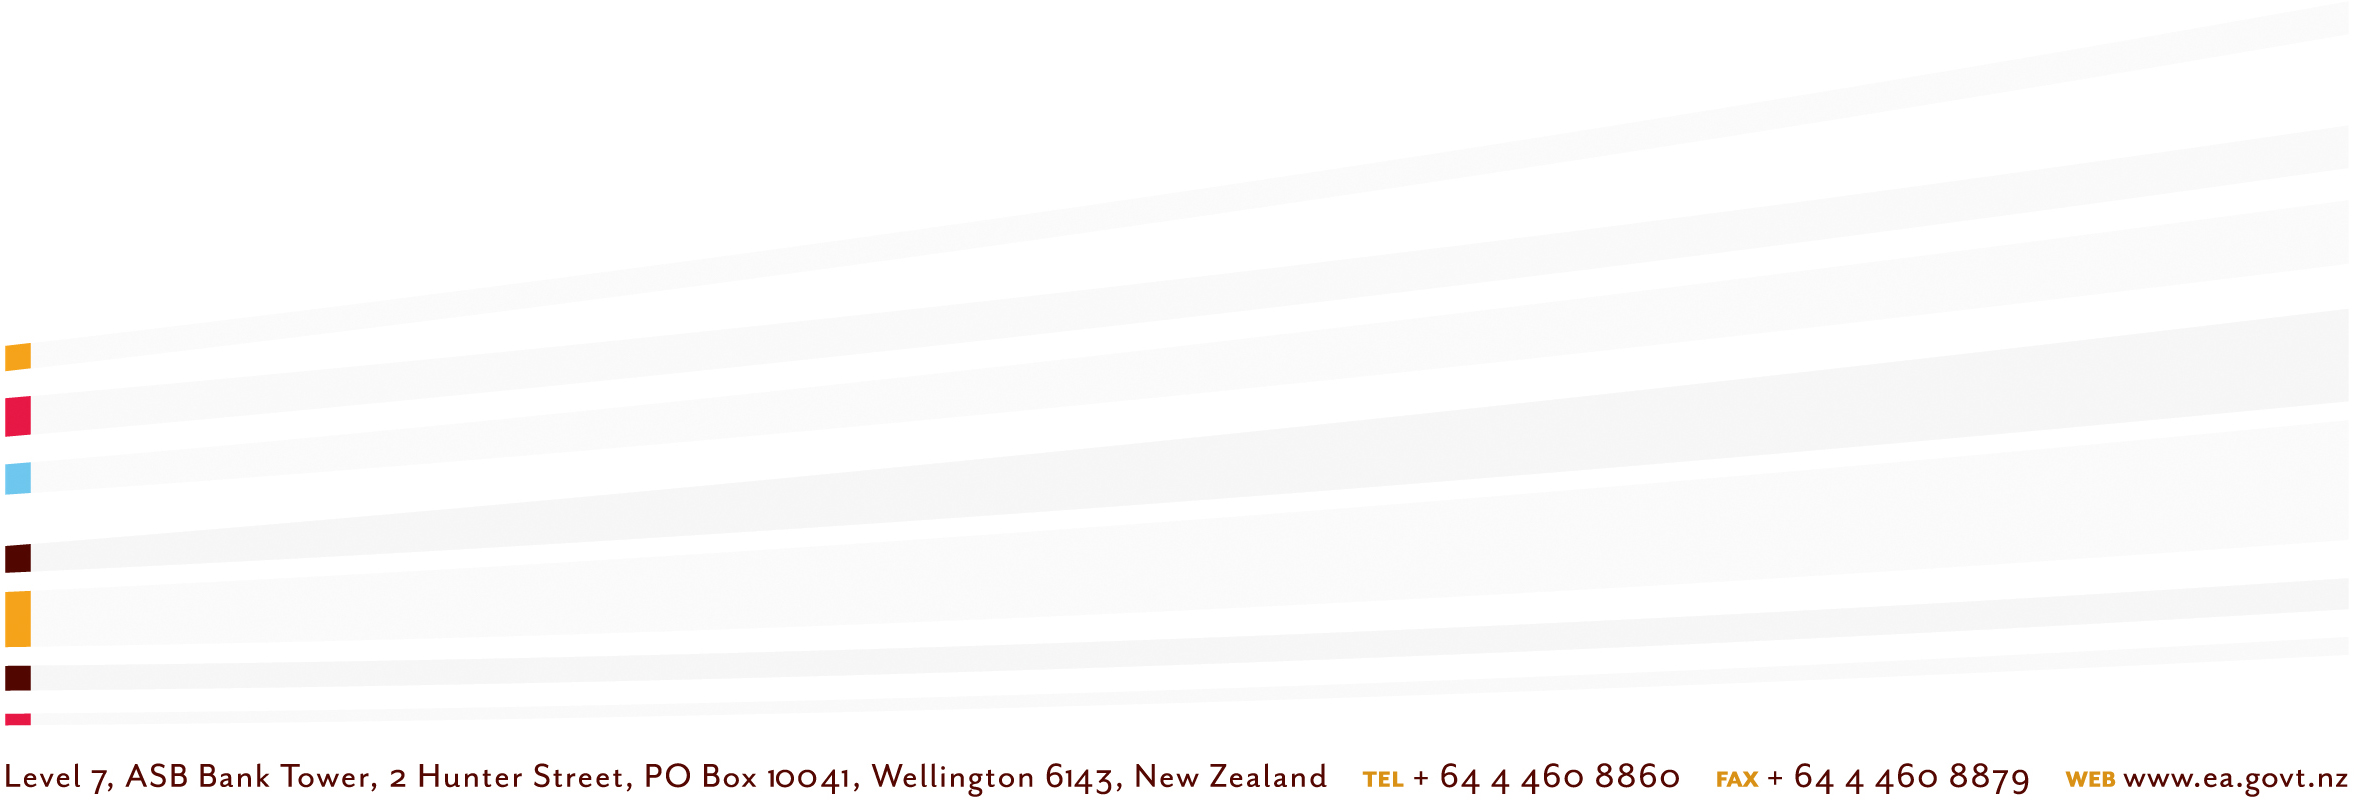
\includegraphics[width=19.75cm]{/home/dave/python/reporting/footer.png}};
\end{tikzpicture}

\begin{tikzpicture}[remember picture,overlay]
    \node (kinmap) [xshift=-0.5cm,yshift=-0.5cm] at (current page.north east) [below left] {
\includegraphics[width=6cm]{/home/dave/python/reporting/ea-logo-medium.jpg}};
\end{tikzpicture}

%\begin{tikzpicture}[remember picture,overlay]
%    \node (kinmap) [xshift=0.5cm,yshift=0.25cm] at (current page.south) [above] {\tiny Compiled: \today \hspace{0.5mm} \currenttime};
%\end{tikzpicture}


\begin{tikzpicture}[remember picture,overlay]
    \node (kinmap) [xshift=1.35cm,yshift=8cm] at (current page.south west) [above right] {
    
    \begin{minipage}{\textwidth}\tiny This document is provided for information purposes only. The Electricity Authority and other parties who have contributed information to this document (Contributing Parties) make no representation or warranty as to the accuracy or completeness of the information contained in this document. The Electricity Authority and the Contributing Parties accept no liability or responsibility for any loss, costs or expenses, of whatever nature arising out of or in connection with the use of this document.

©ASX Limited ABN 98 008 624 691 (ASX) 2012. All rights reserved. ASX information is reproduced with the permission of ASX. ASX information should not be reproduced, stored in a retrieval system or transmitted in any form whether in whole or in part without the prior
written permission of ASX.

The information in this document does not constitute personalised financial advice. While the Authority has made every effort to ensure that the information provided is accurate, you should not rely on this information to make any financial decisions. If you are a considering taking an exposure to
electricity spot prices or to financial derivatives referenced to electricity spot prices, you should carefully consider the risks and benefits and, if necessary, seek professional advice.
\end{minipage}
};
\end{tikzpicture}






\newpage


\section{Hydro Risk Curves and current storage situation}
\vspace{1cm}
\begin{center}
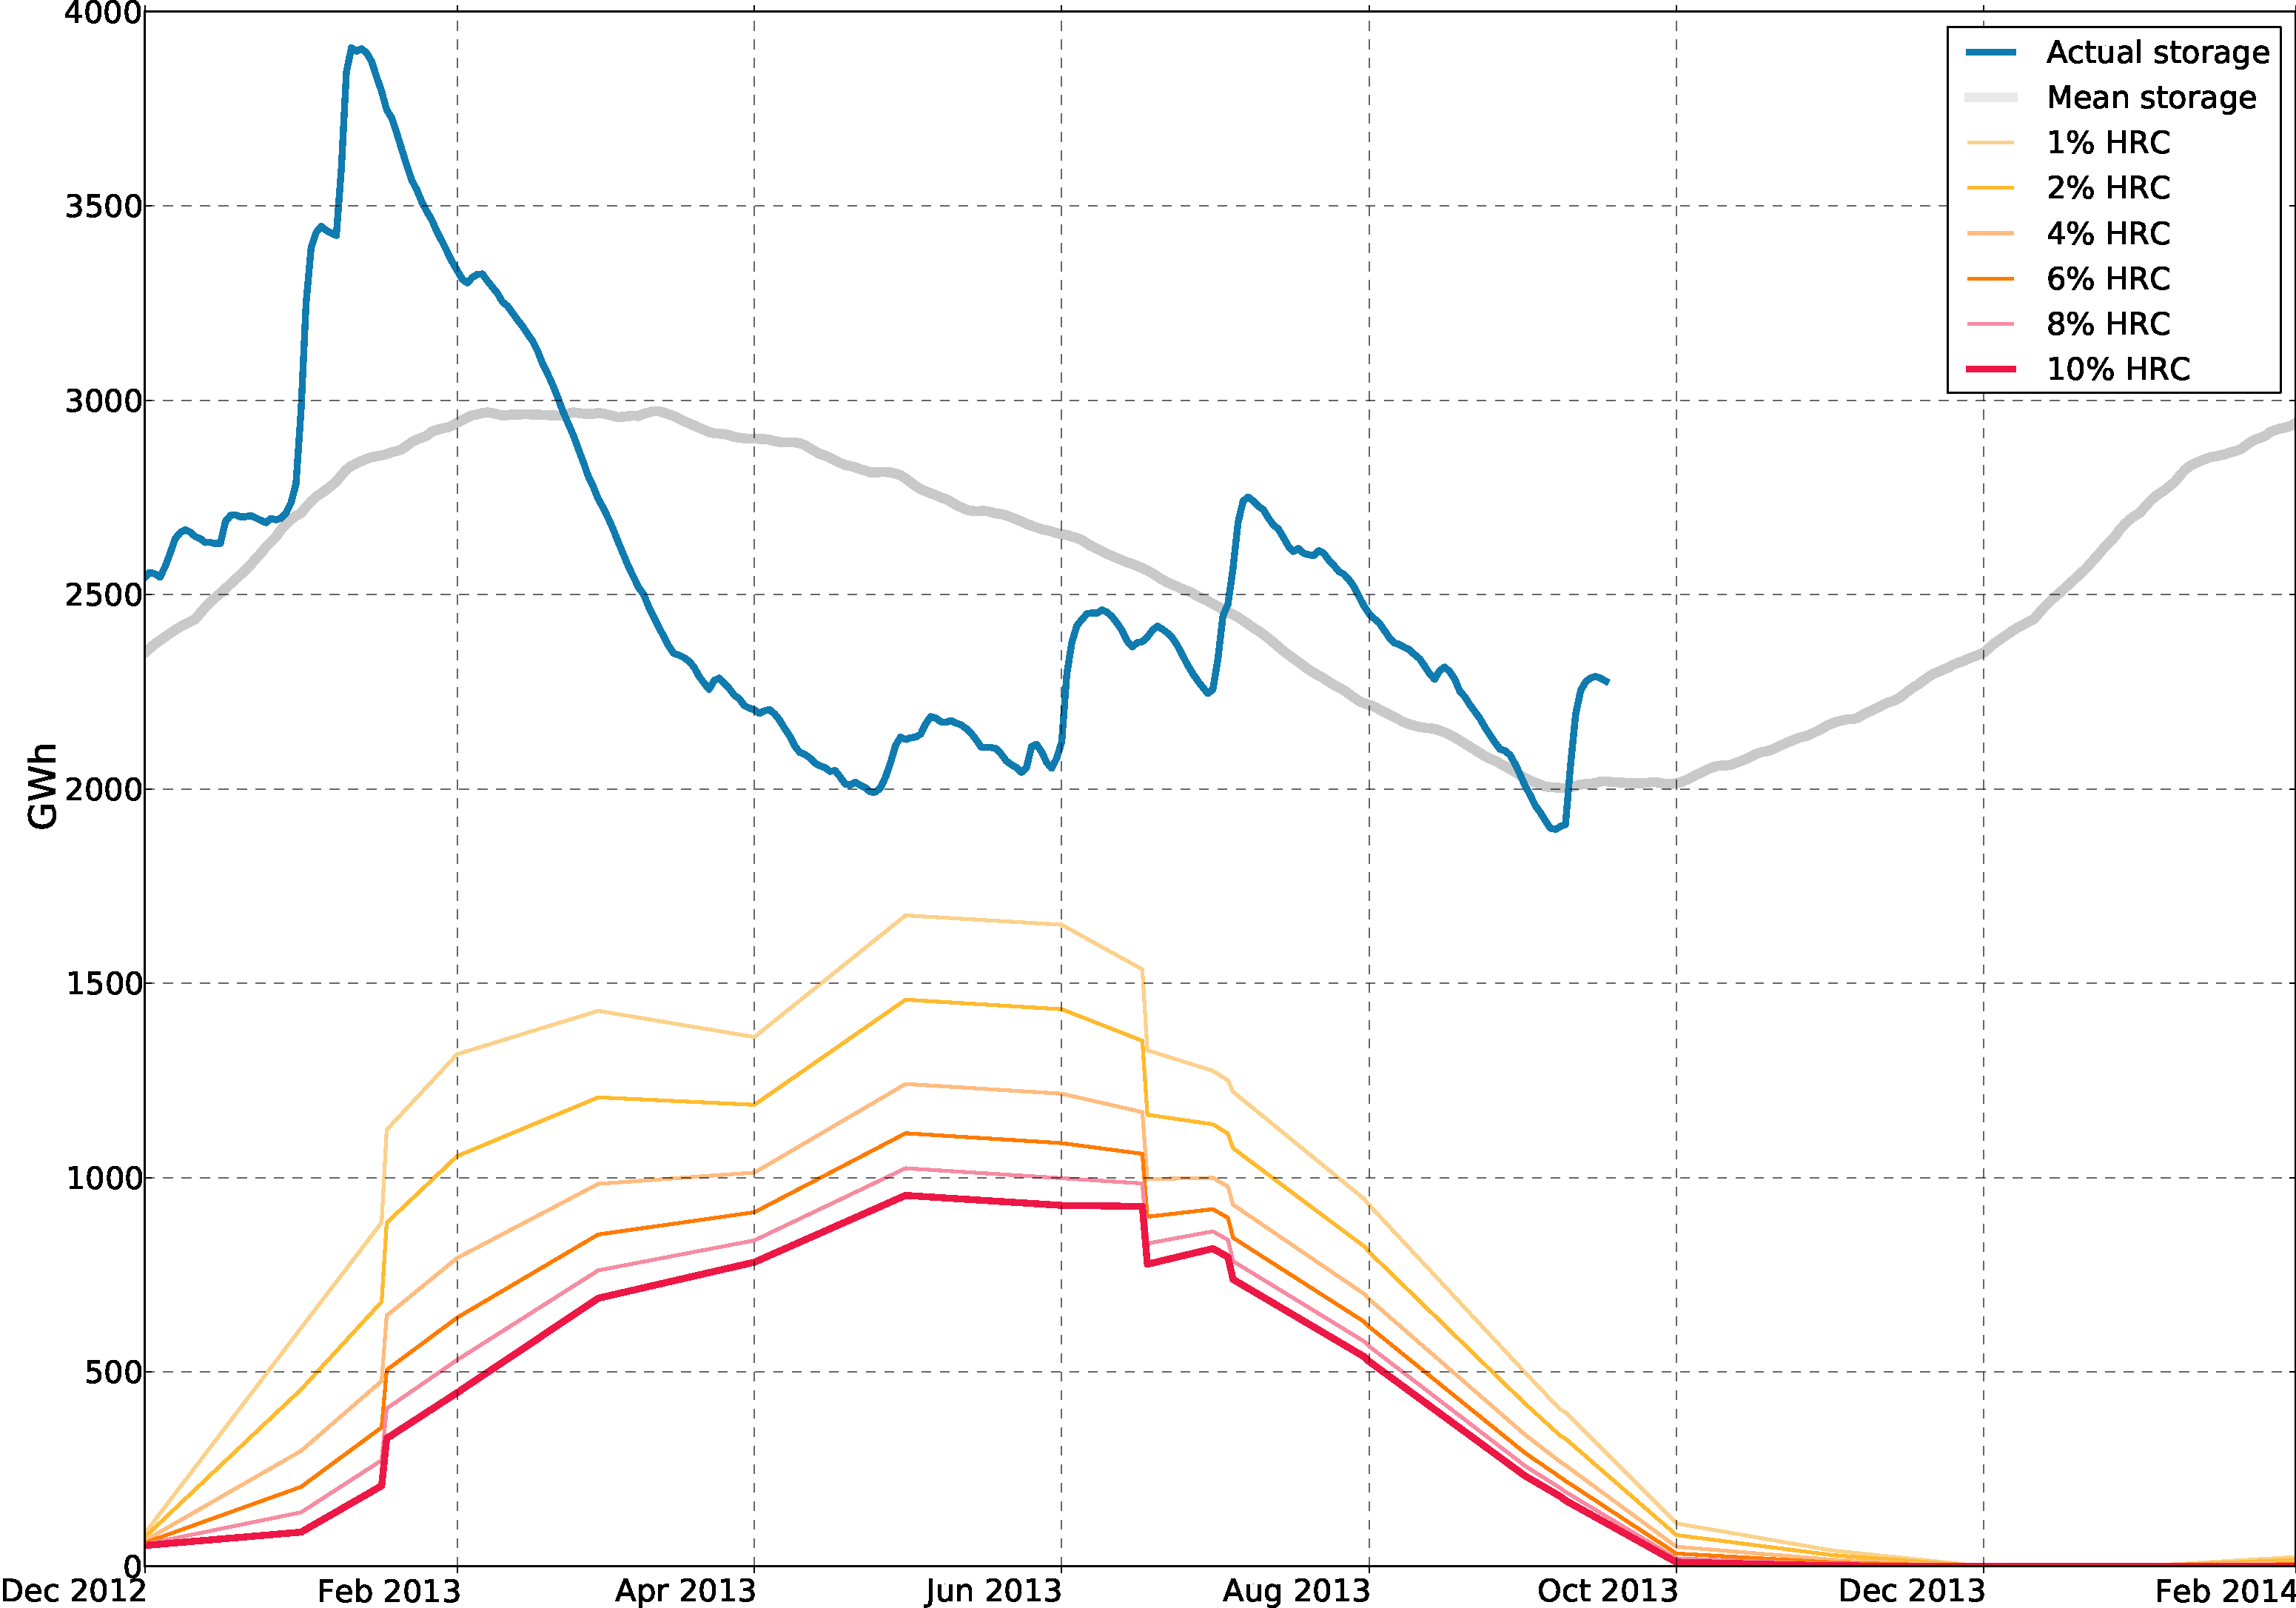
\includegraphics[max size={\textwidth}{0.9\textheight}]{/home/dave/python/reporting/figures/hrc.pdf}
\end{center}

\scriptsize Source: HRCs:Electricity Authority/System Operator, Hydro data \url{ http://www.comithydro.niwa.co.nz/}



\subsection{NZ total storage and inflows over past year}
\vspace{5mm}

\begin{center}
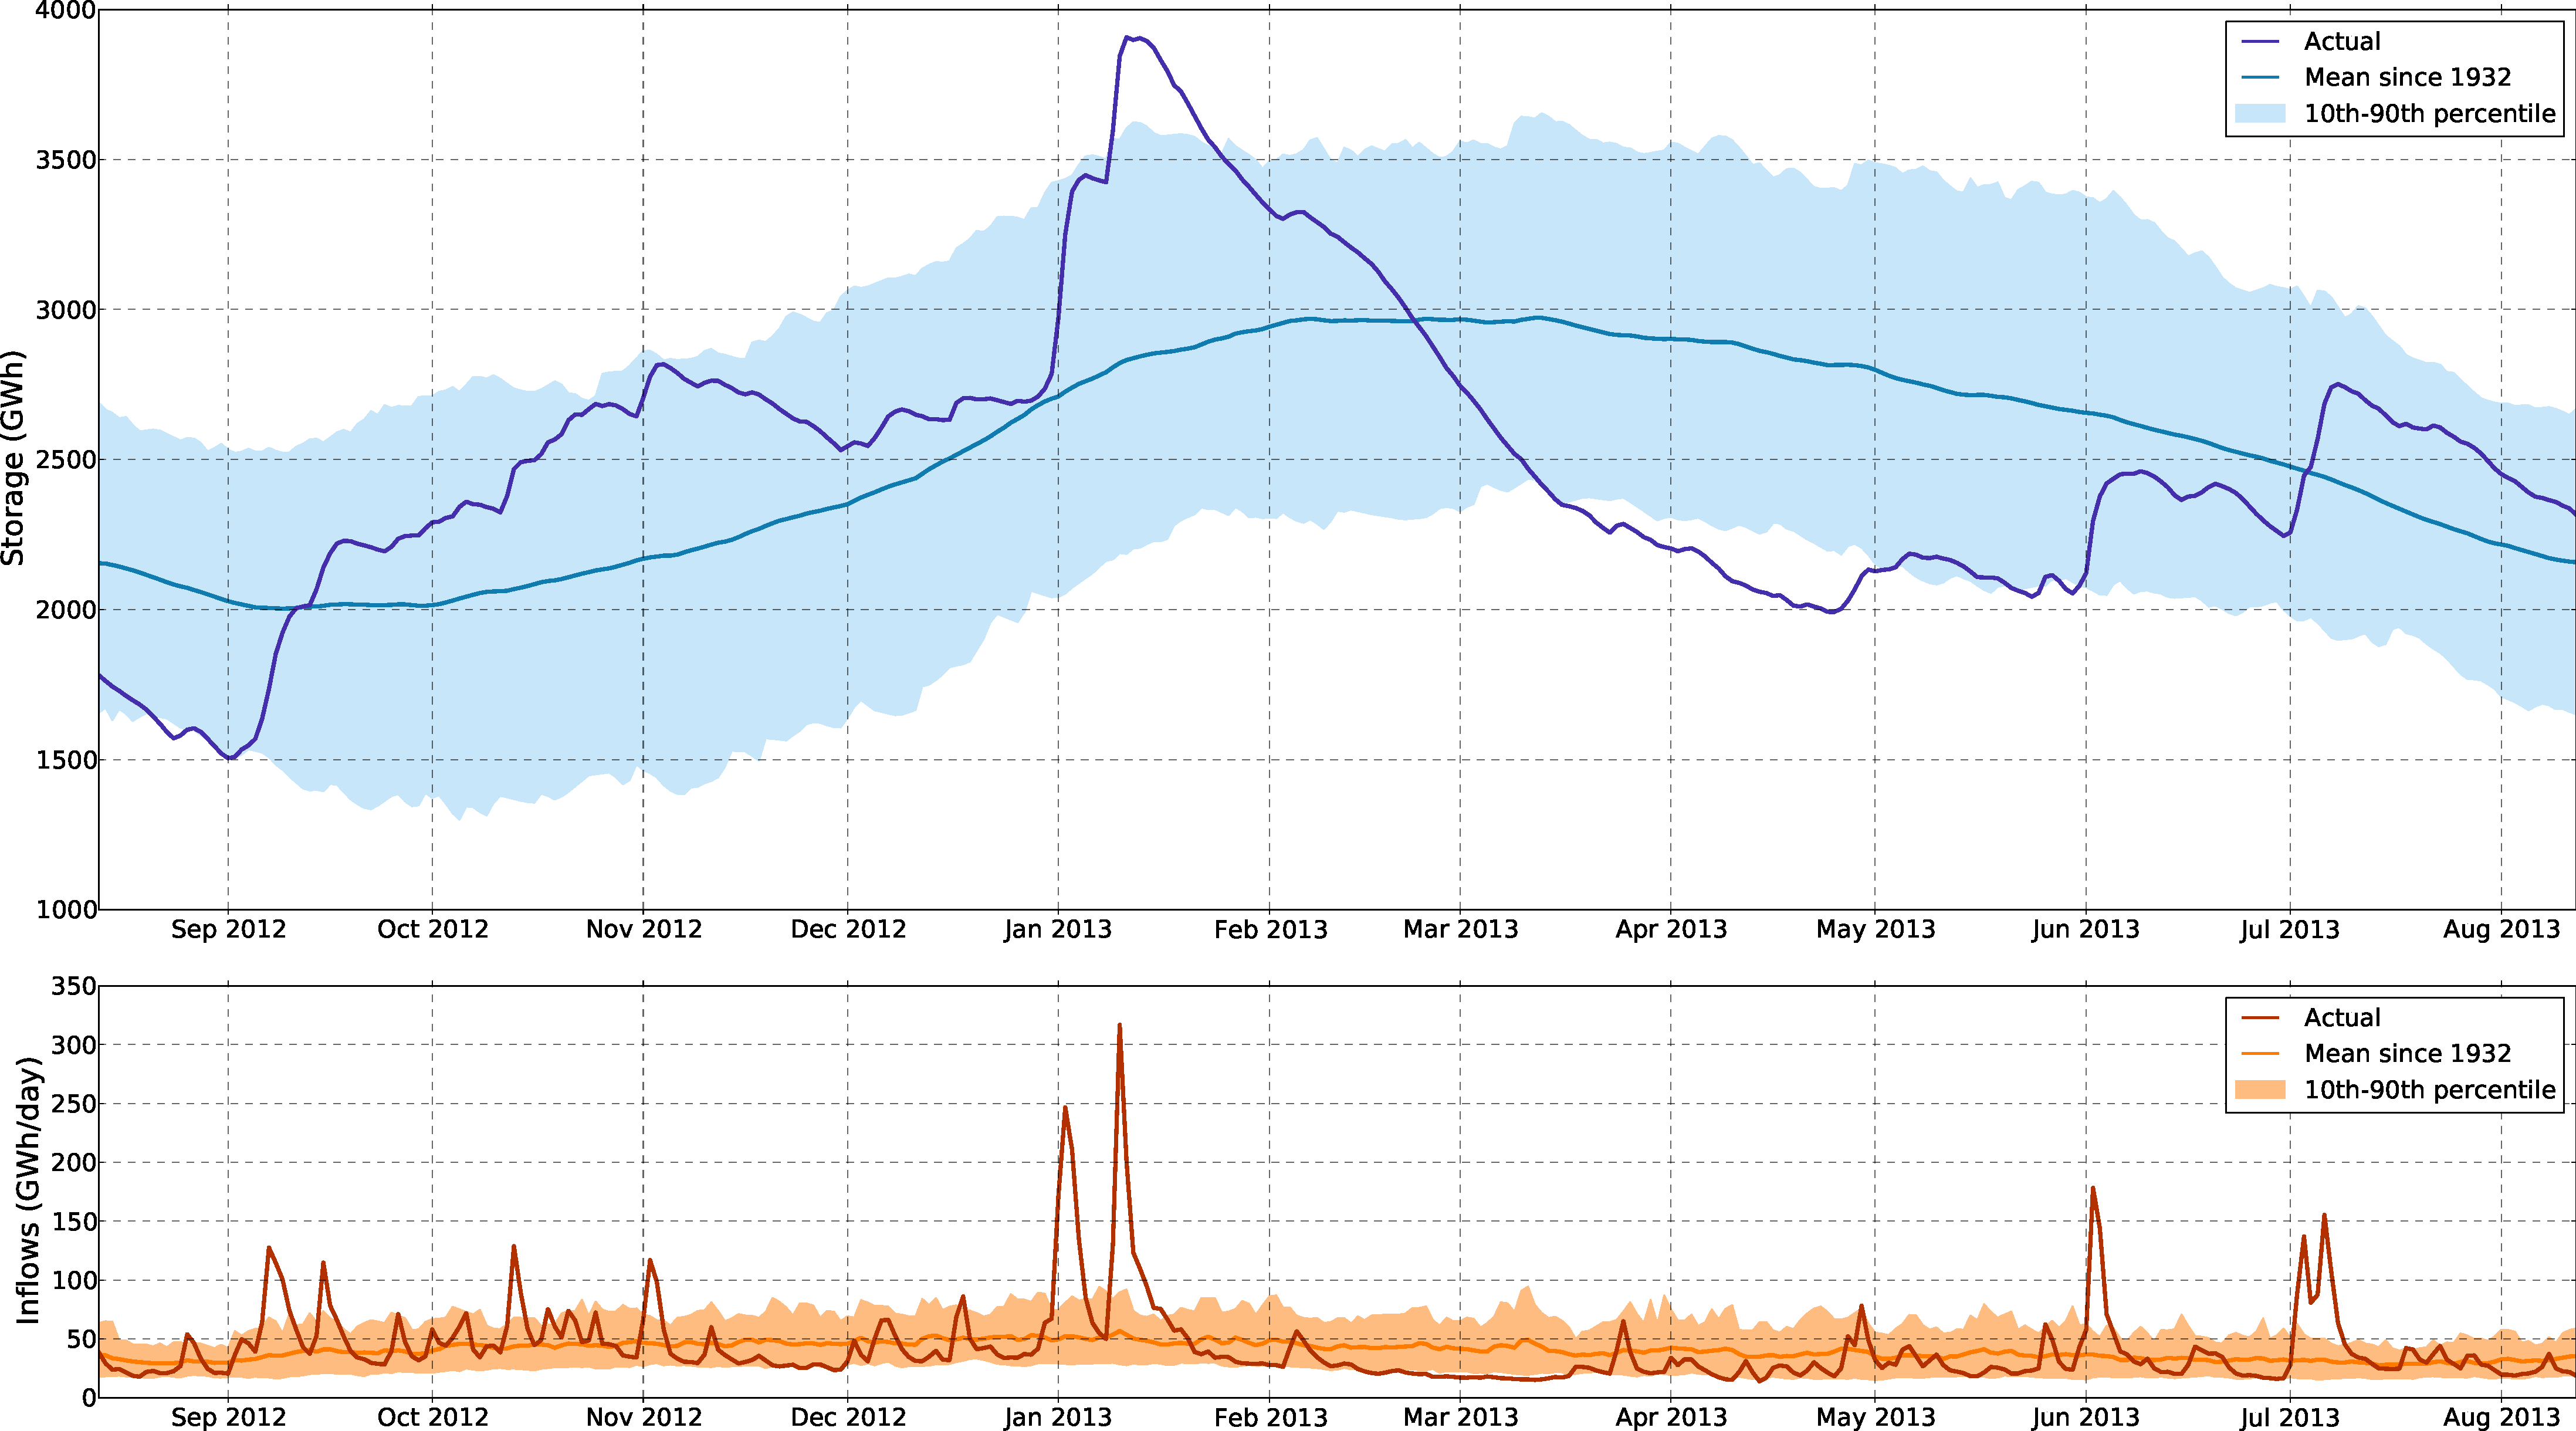
\includegraphics[max size={\textwidth}{0.9\textheight}]{/home/dave/python/reporting/figures/nz.pdf}
\end{center}
\scriptsize Source: Electricity Authority/Comit Hydro 

\vspace{5mm}

\subsection{Lake Taupo total storage and inflows over past year}
\begin{center}
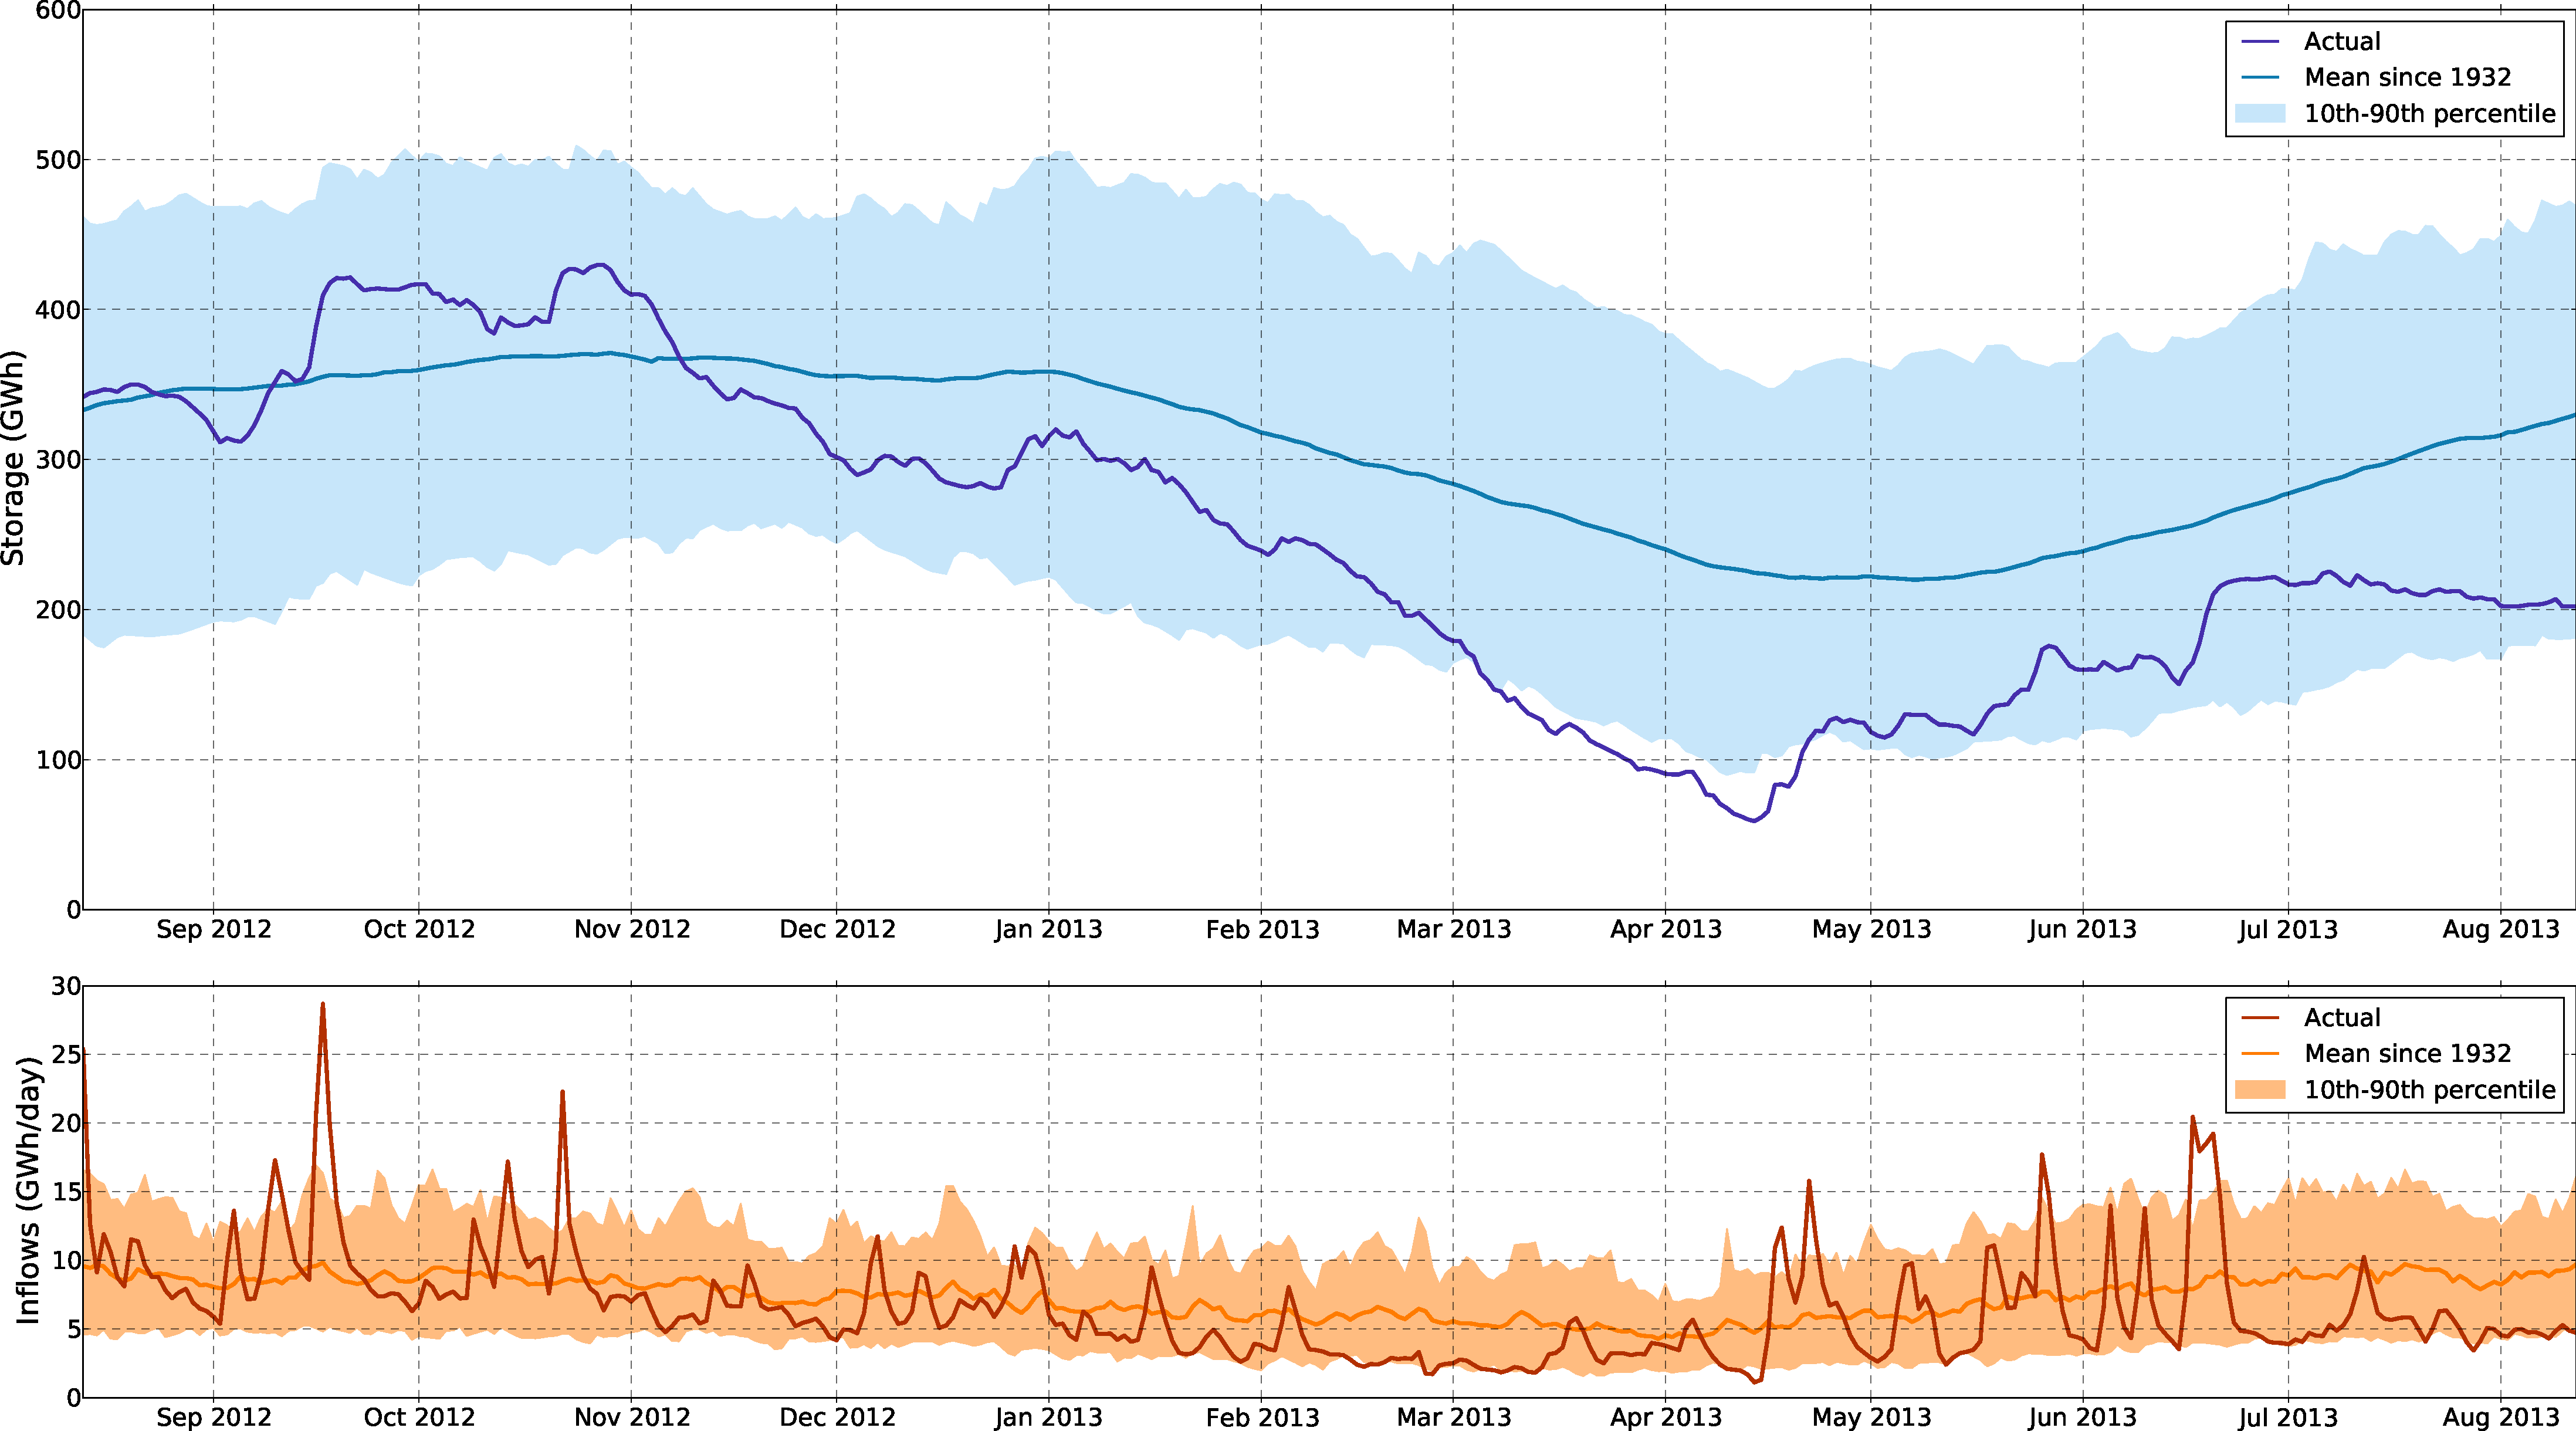
\includegraphics[max size={\textwidth}{0.9\textheight}]{/home/dave/python/reporting/figures/taupo.pdf}
\end{center}


\subsection{Lake Tekapo total storage and inflows over past year}
\begin{center}
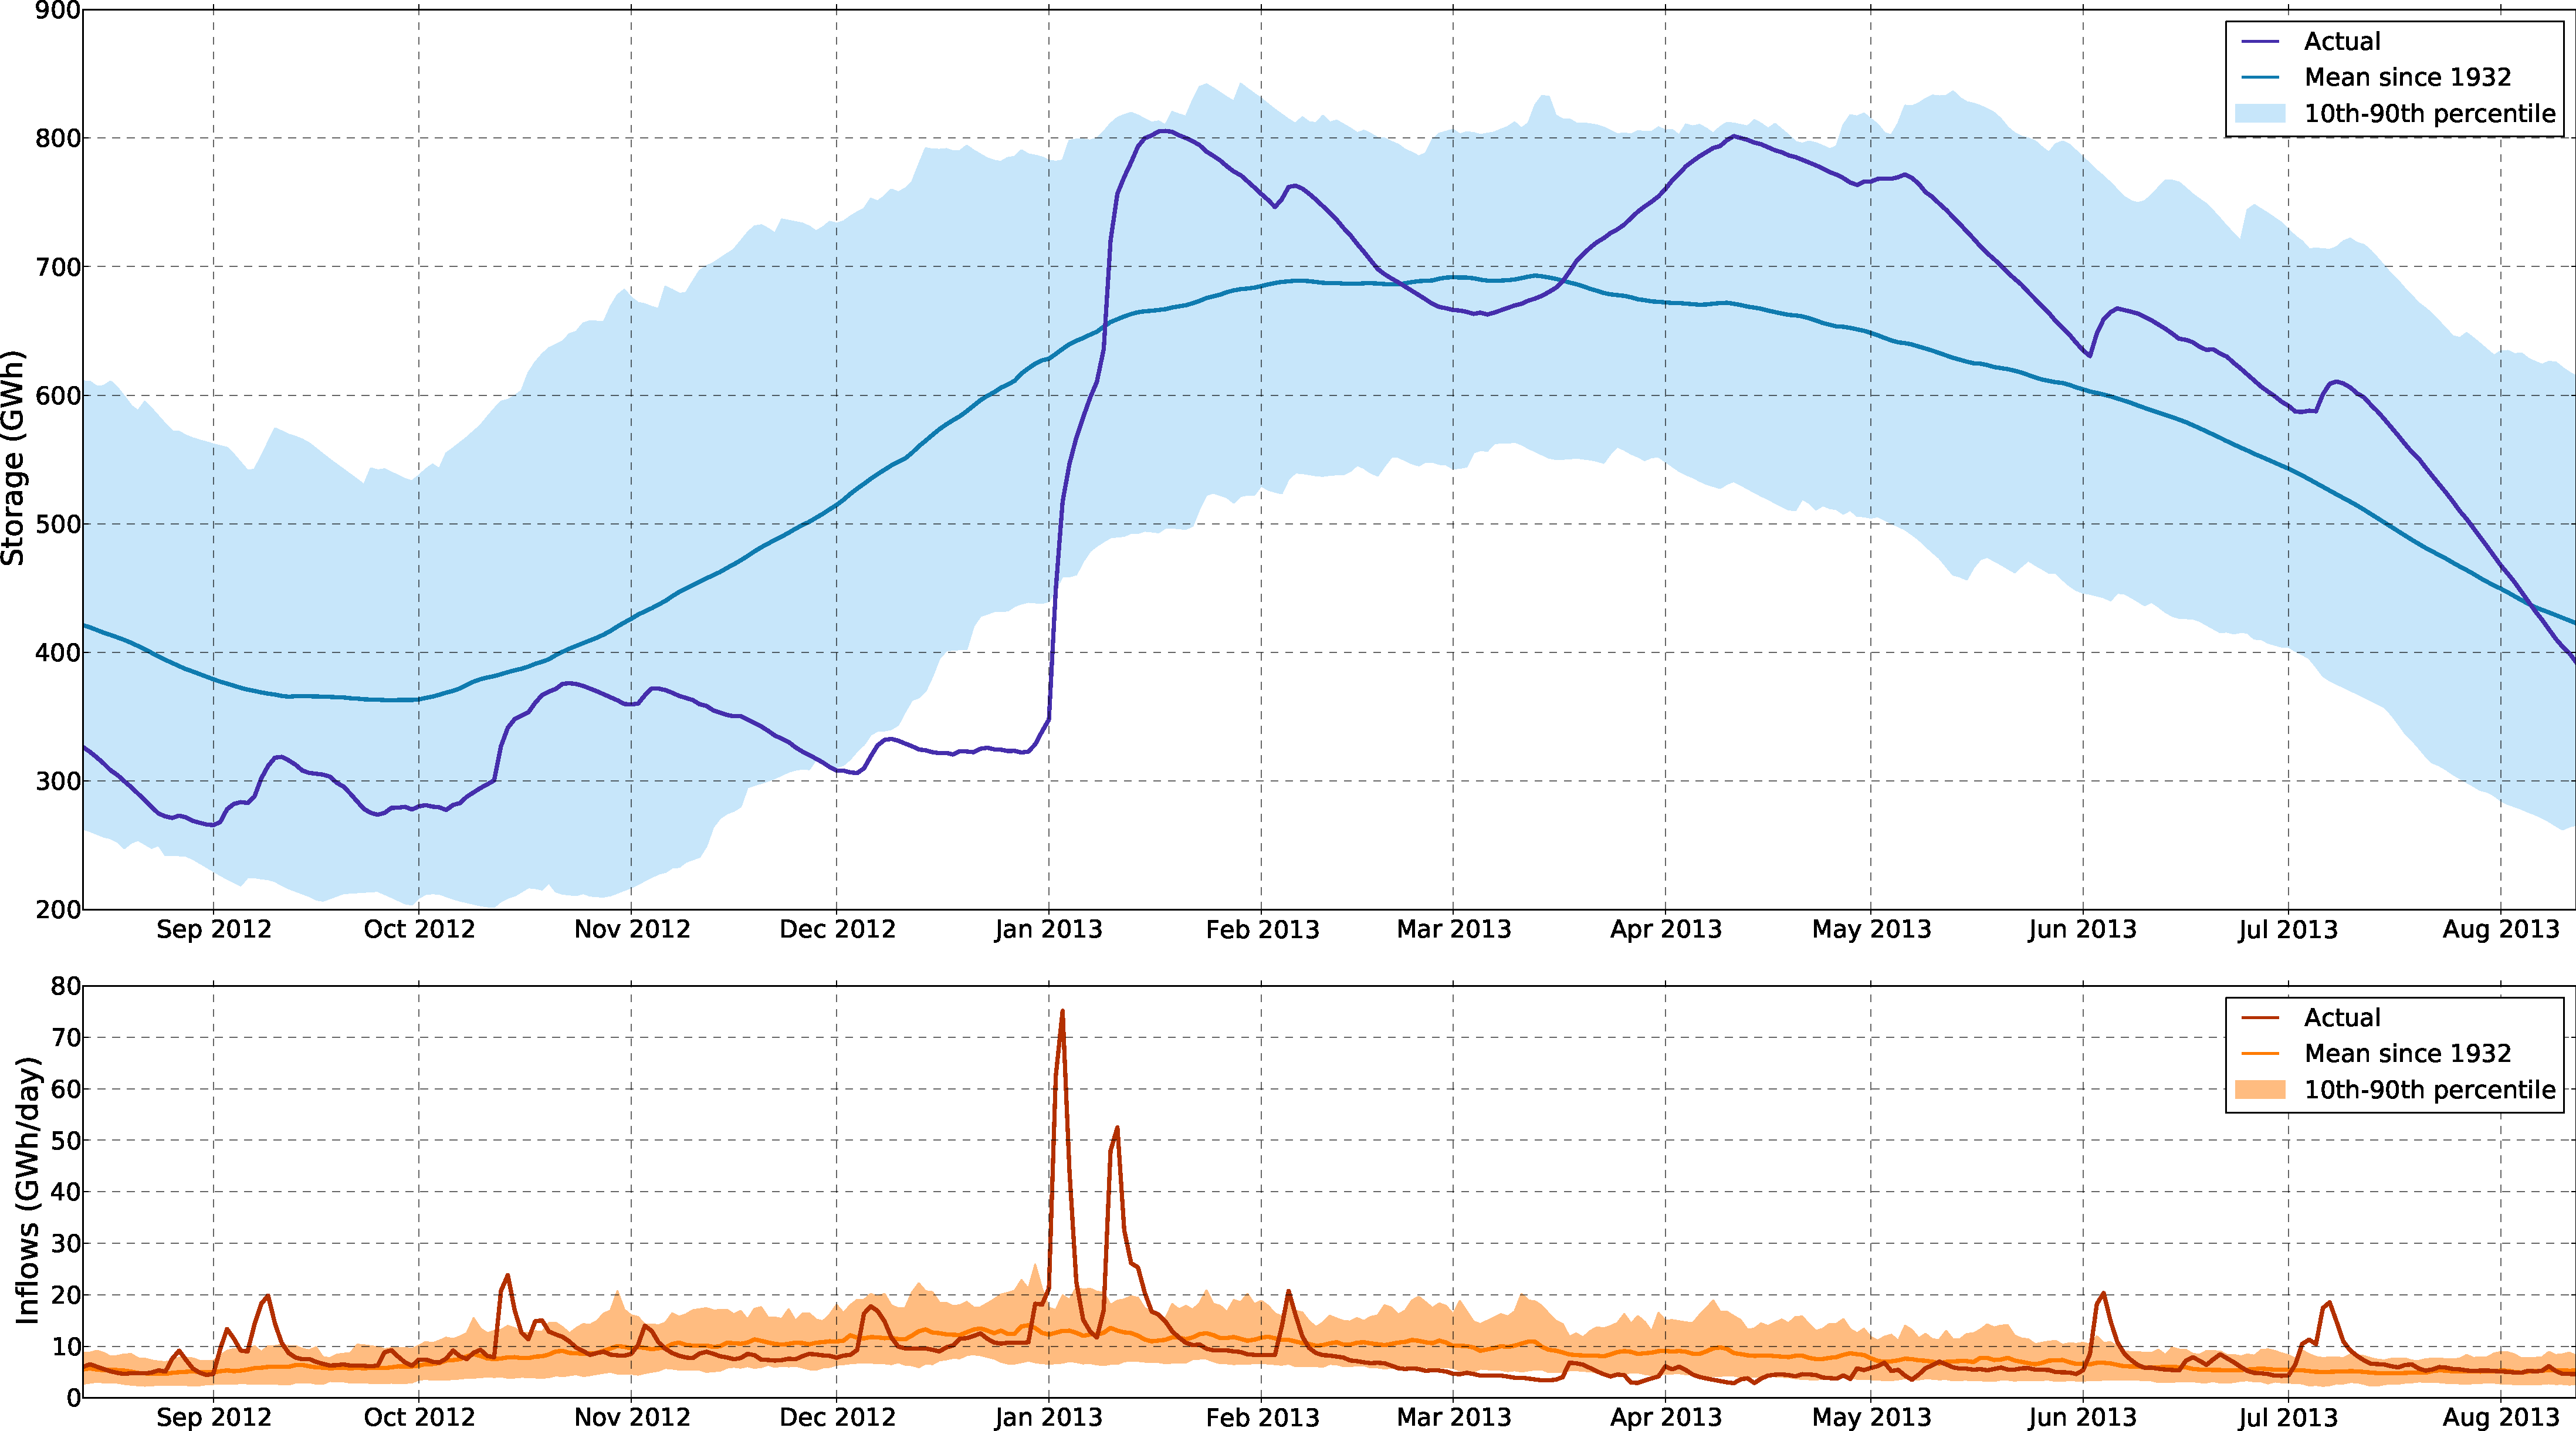
\includegraphics[max size={\textwidth}{0.9\textheight}]{/home/dave/python/reporting/figures/tekapo.pdf}
\end{center}

\vspace{5mm}

\subsection{Lake Pukaki total storage and inflows over past year}
\begin{center}
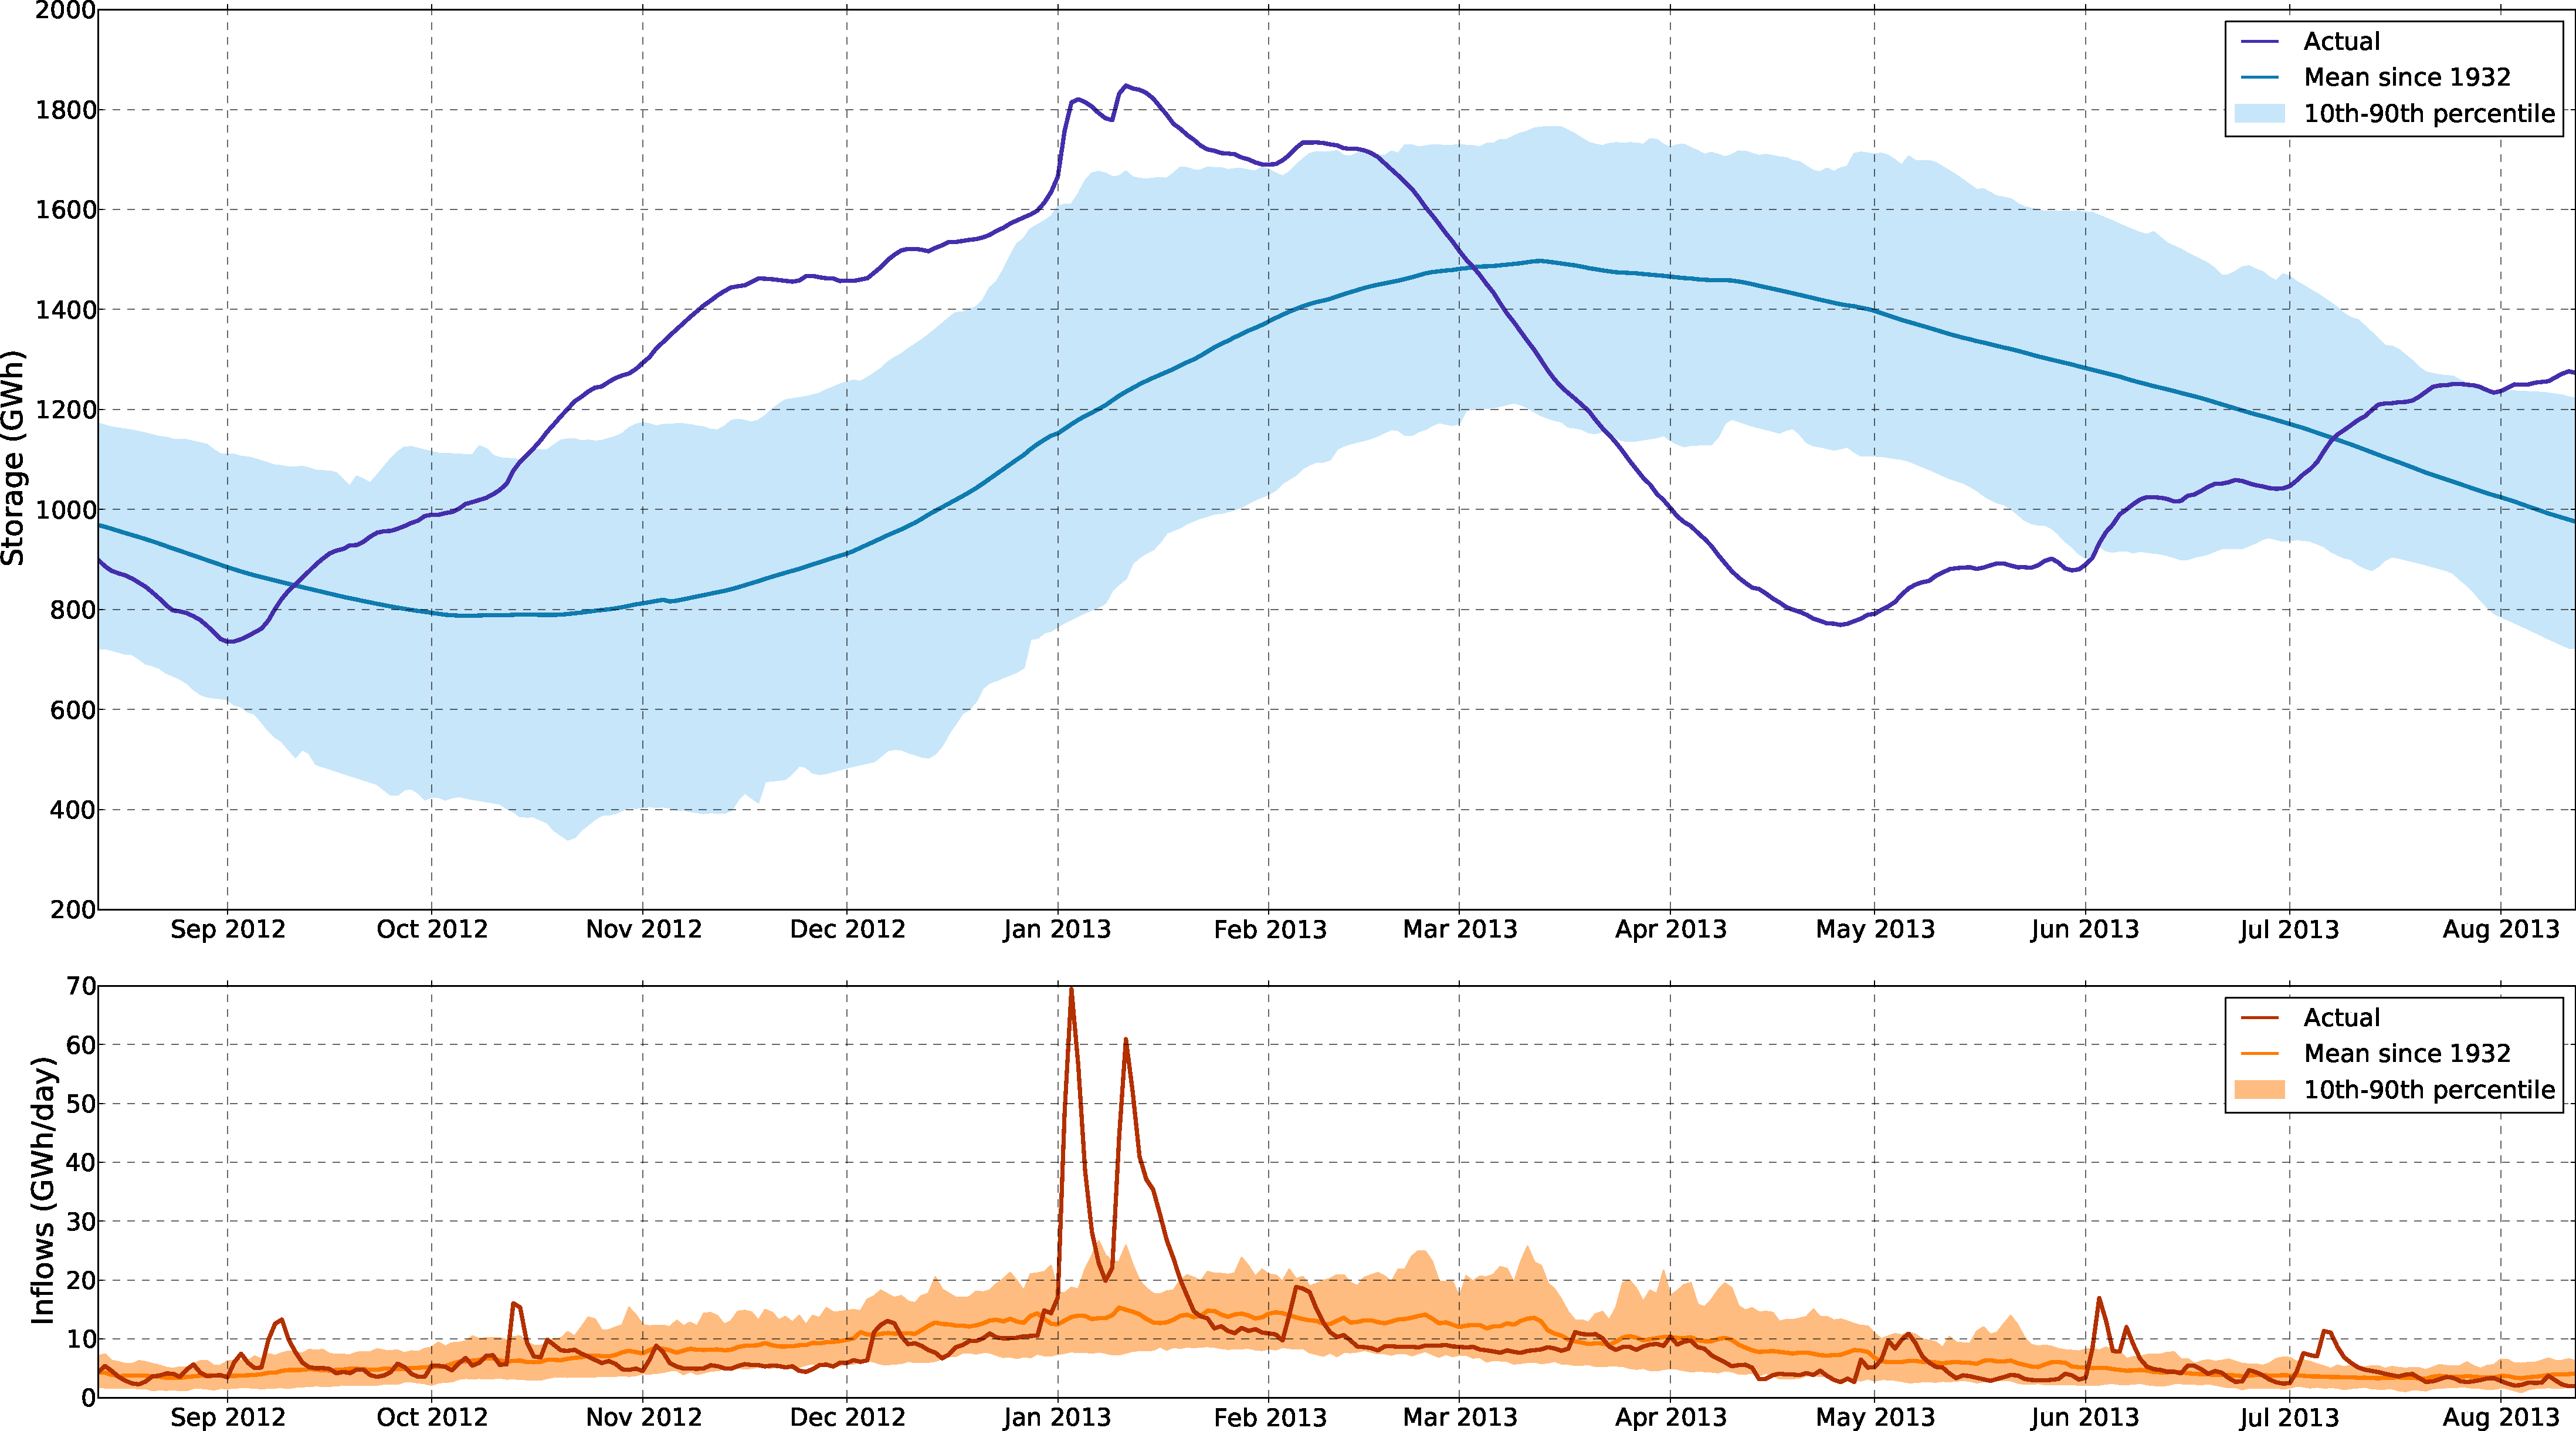
\includegraphics[max size={\textwidth}{0.9\textheight}]{/home/dave/python/reporting/figures/pukaki.pdf}
\end{center}


\subsection{Lake Hawea total storage and inflows over past year}
\vspace{5mm}

\begin{center}
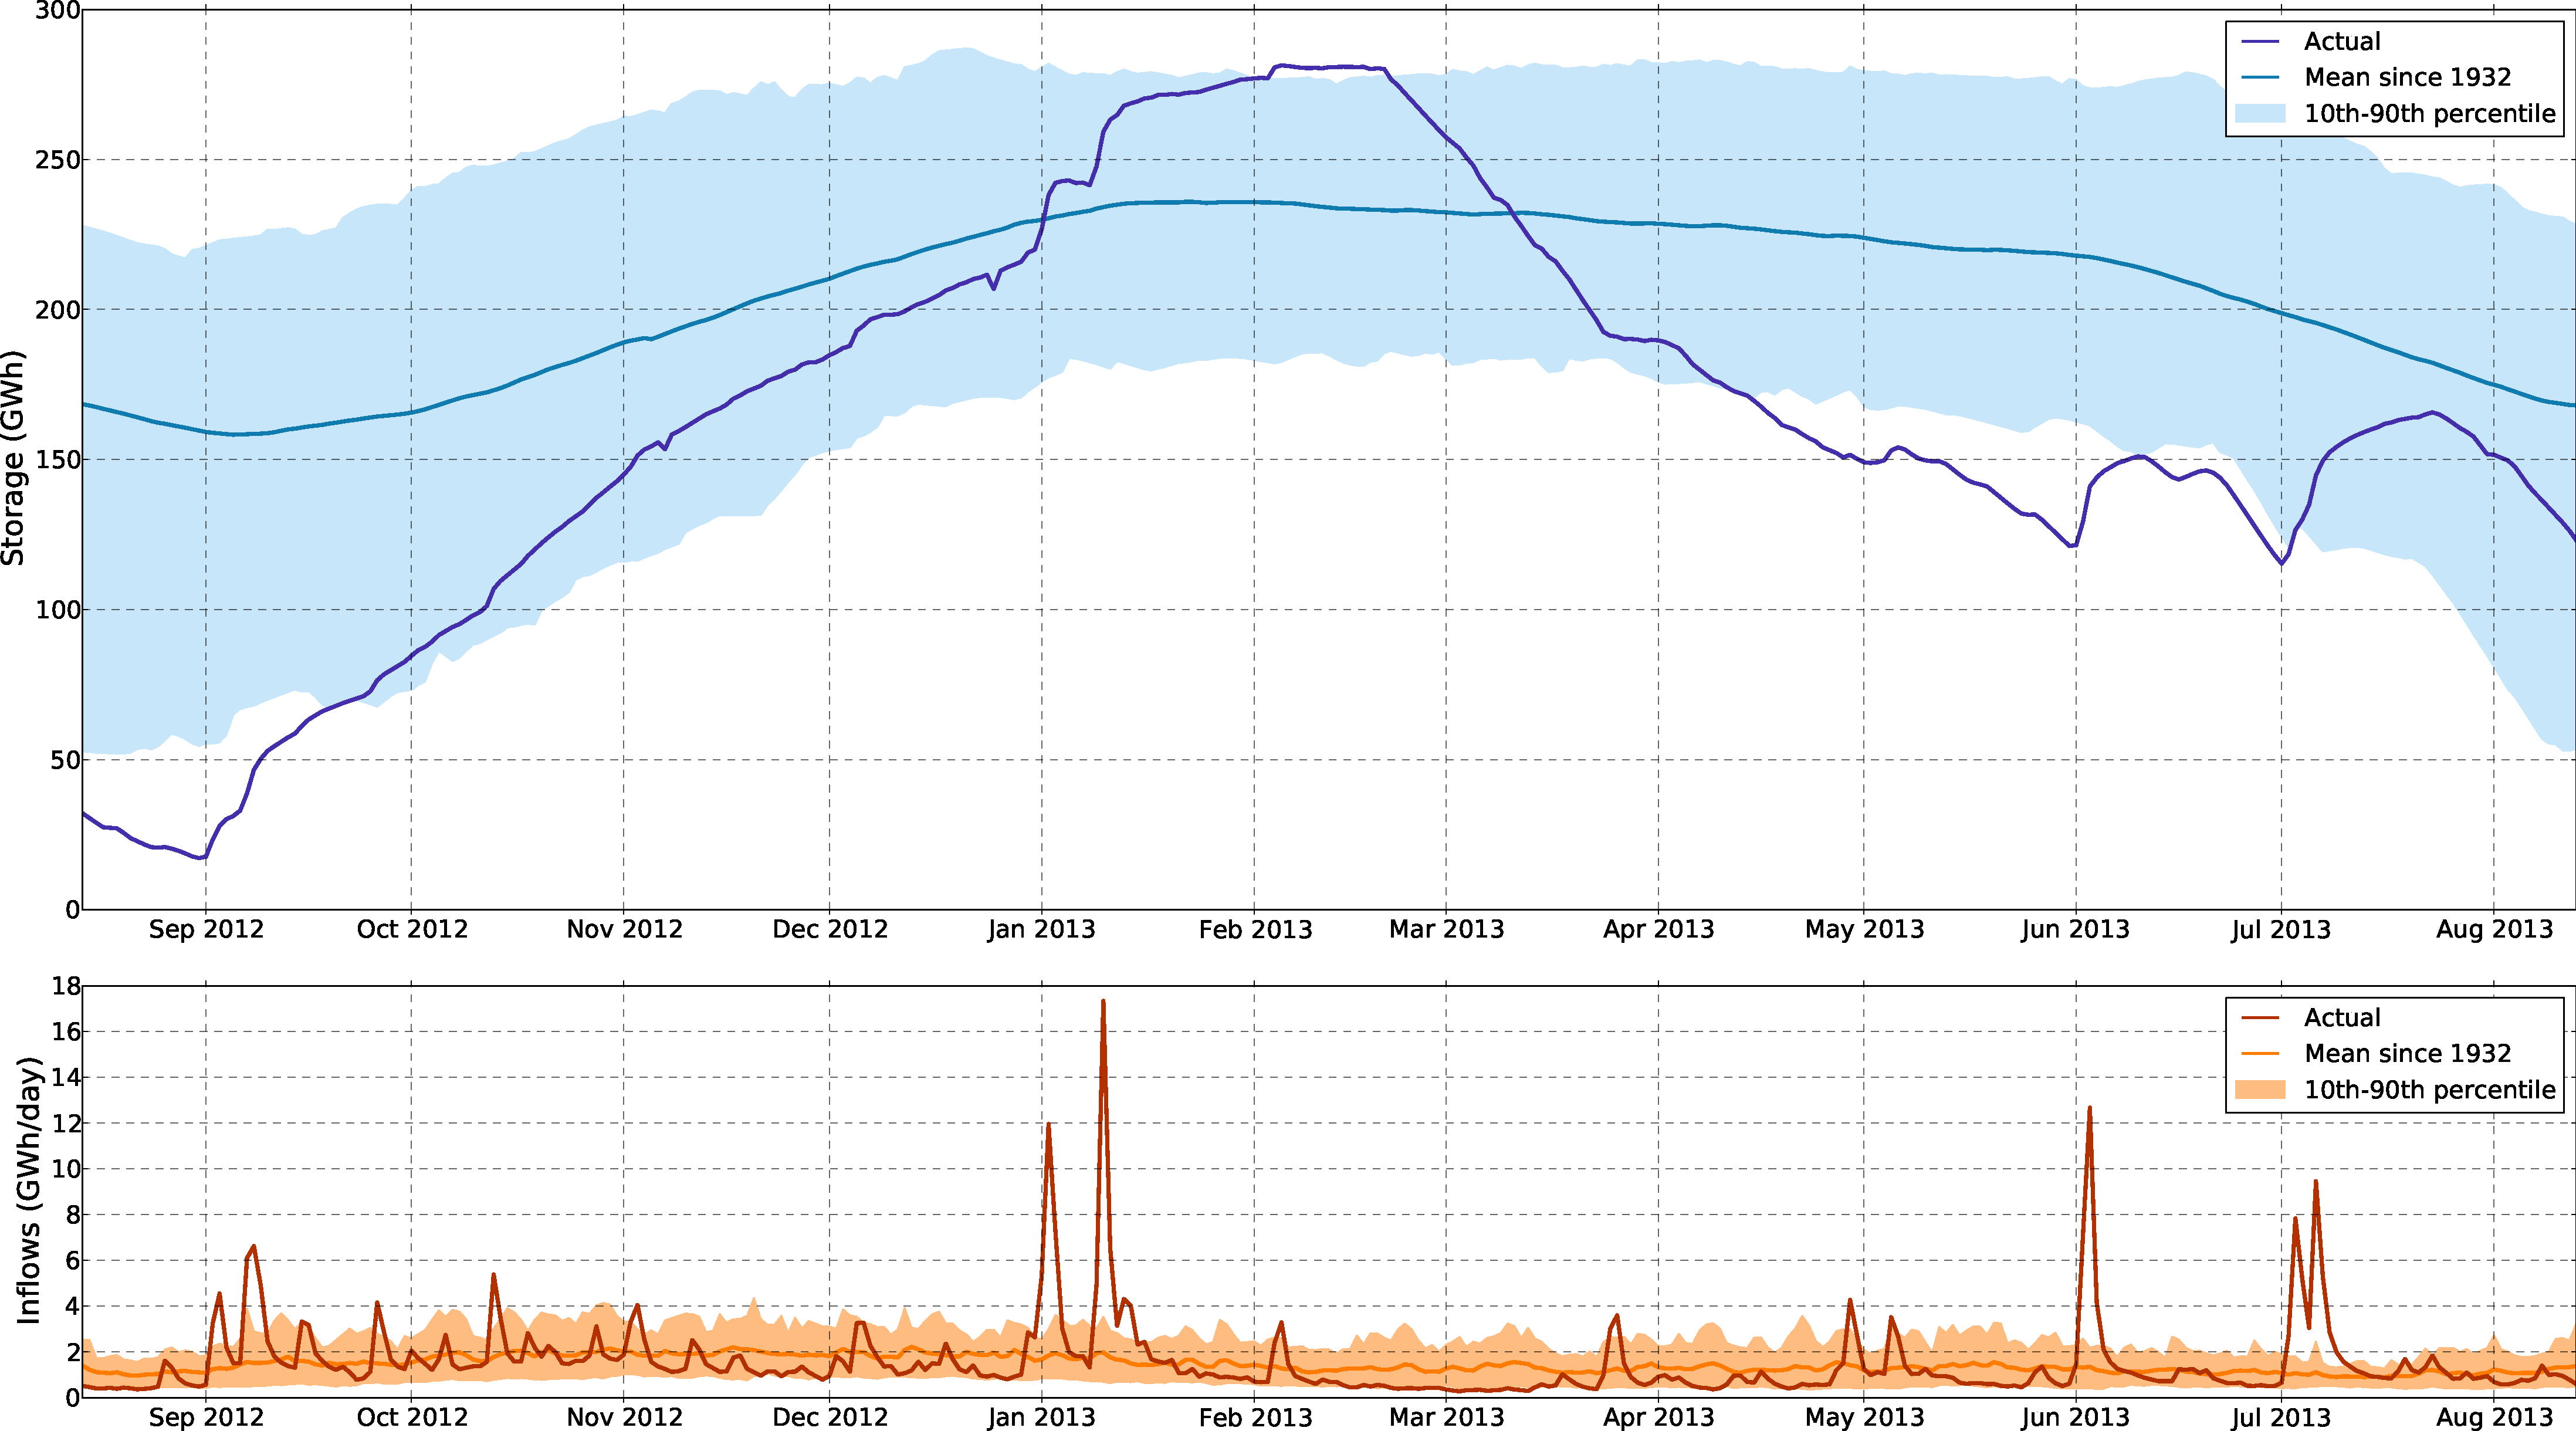
\includegraphics[max size={\textwidth}{0.9\textheight}]{/home/dave/python/reporting/figures/hawea.pdf}
\end{center}

\vspace{5mm}

\subsection{Lake Te Anau and Manapouri total storage and inflows over
past year}
\begin{center}
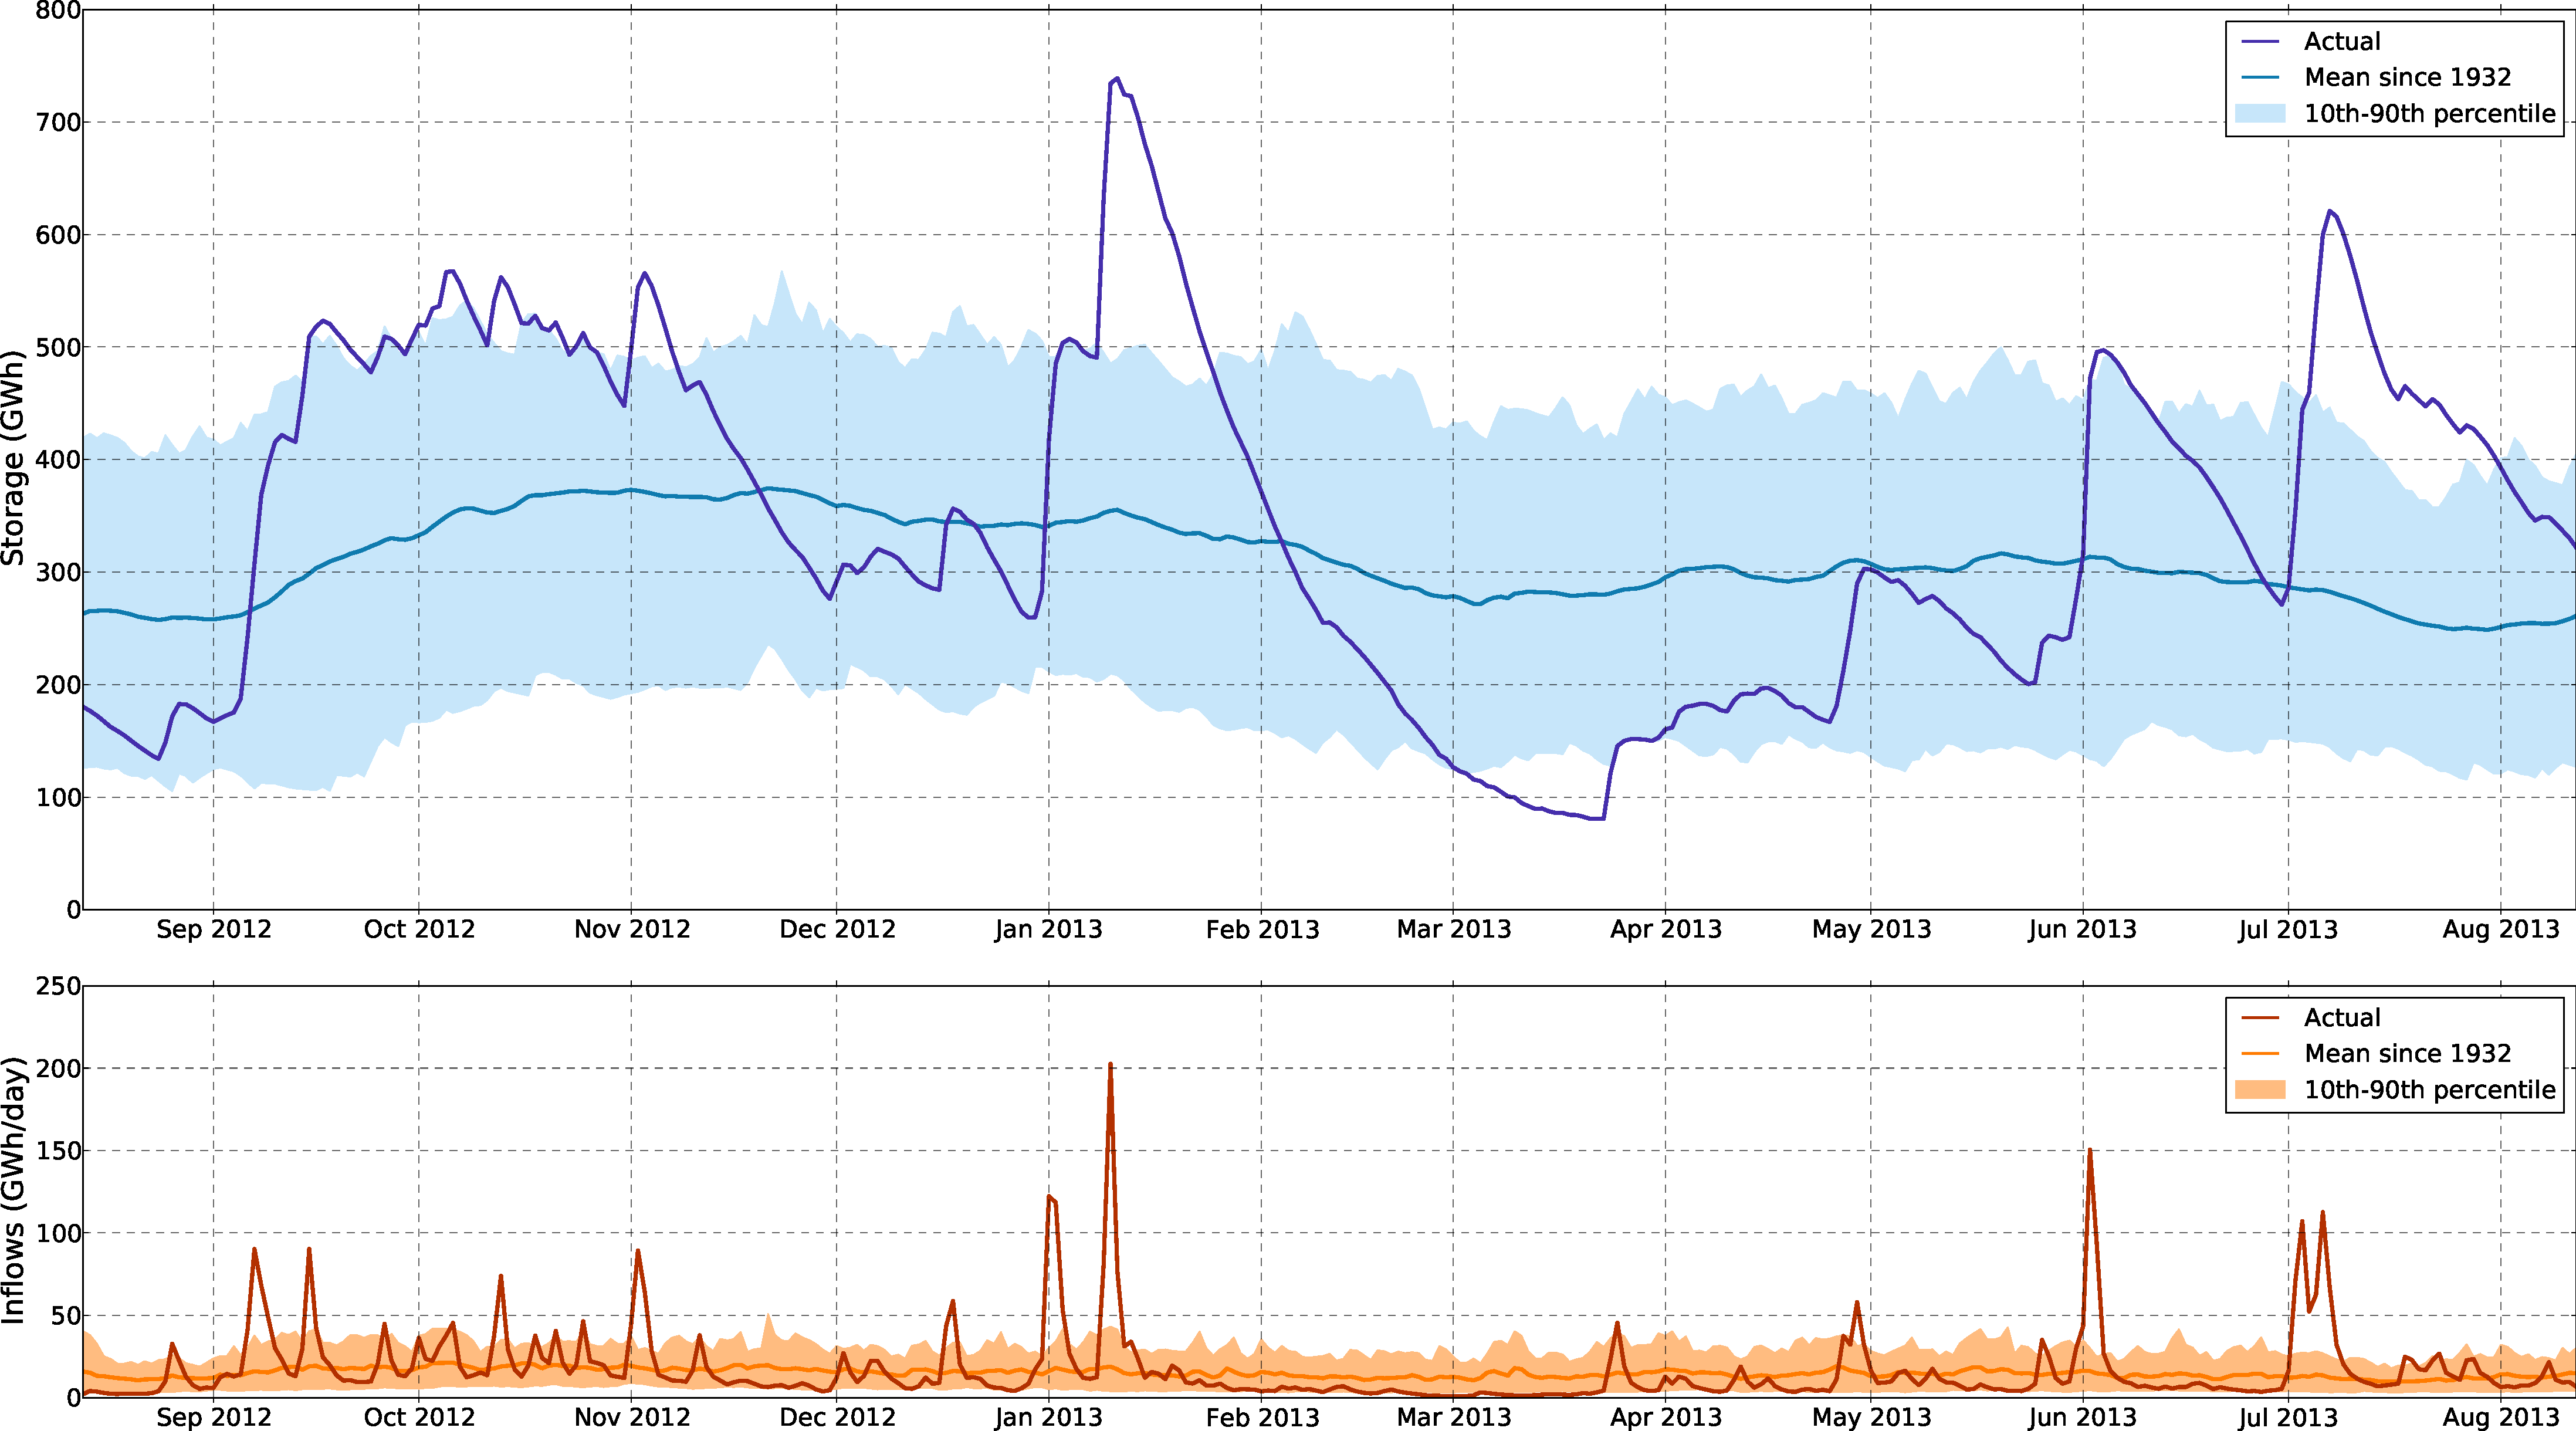
\includegraphics[max size={\textwidth}{0.9\textheight}]{/home/dave/python/reporting/figures/teanaumanapouri.pdf}
\end{center}

\subsection{Snow Storage}
\begin{center}
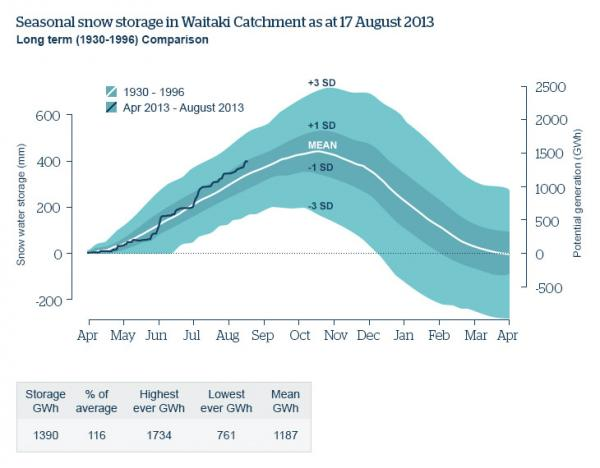
\includegraphics[max size={0.8\textwidth}{0.8\textheight}]{/home/dave/python/reporting/figures/snow.png}
\end{center}
\scriptsize Source: \url{http://www.meridianenergy.co.nz/about-us/generating-energy/lake-levels-and-snow-storage/snow-storage/}

\subsection{Rainfall outlook}
\begin{center}
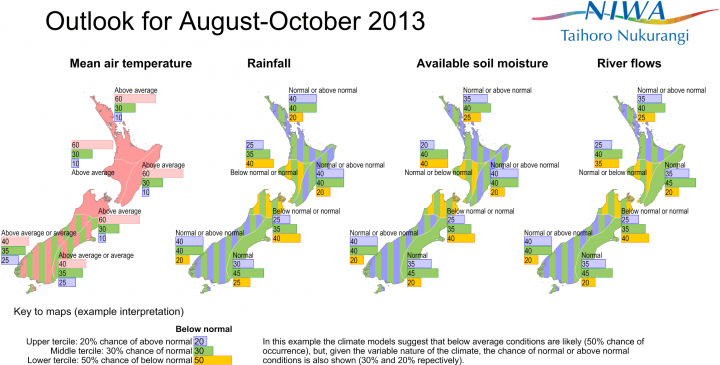
\includegraphics[max size={\textwidth}{0.9\textheight}]{/home/dave/python/reporting/figures/niwa.png}
\end{center}
\scriptsize Source: \url{http://www.niwa.co.nz/climate/sco}


\section{Three month demand weighted price comparison}
\vspace{2cm}

\begin{center}
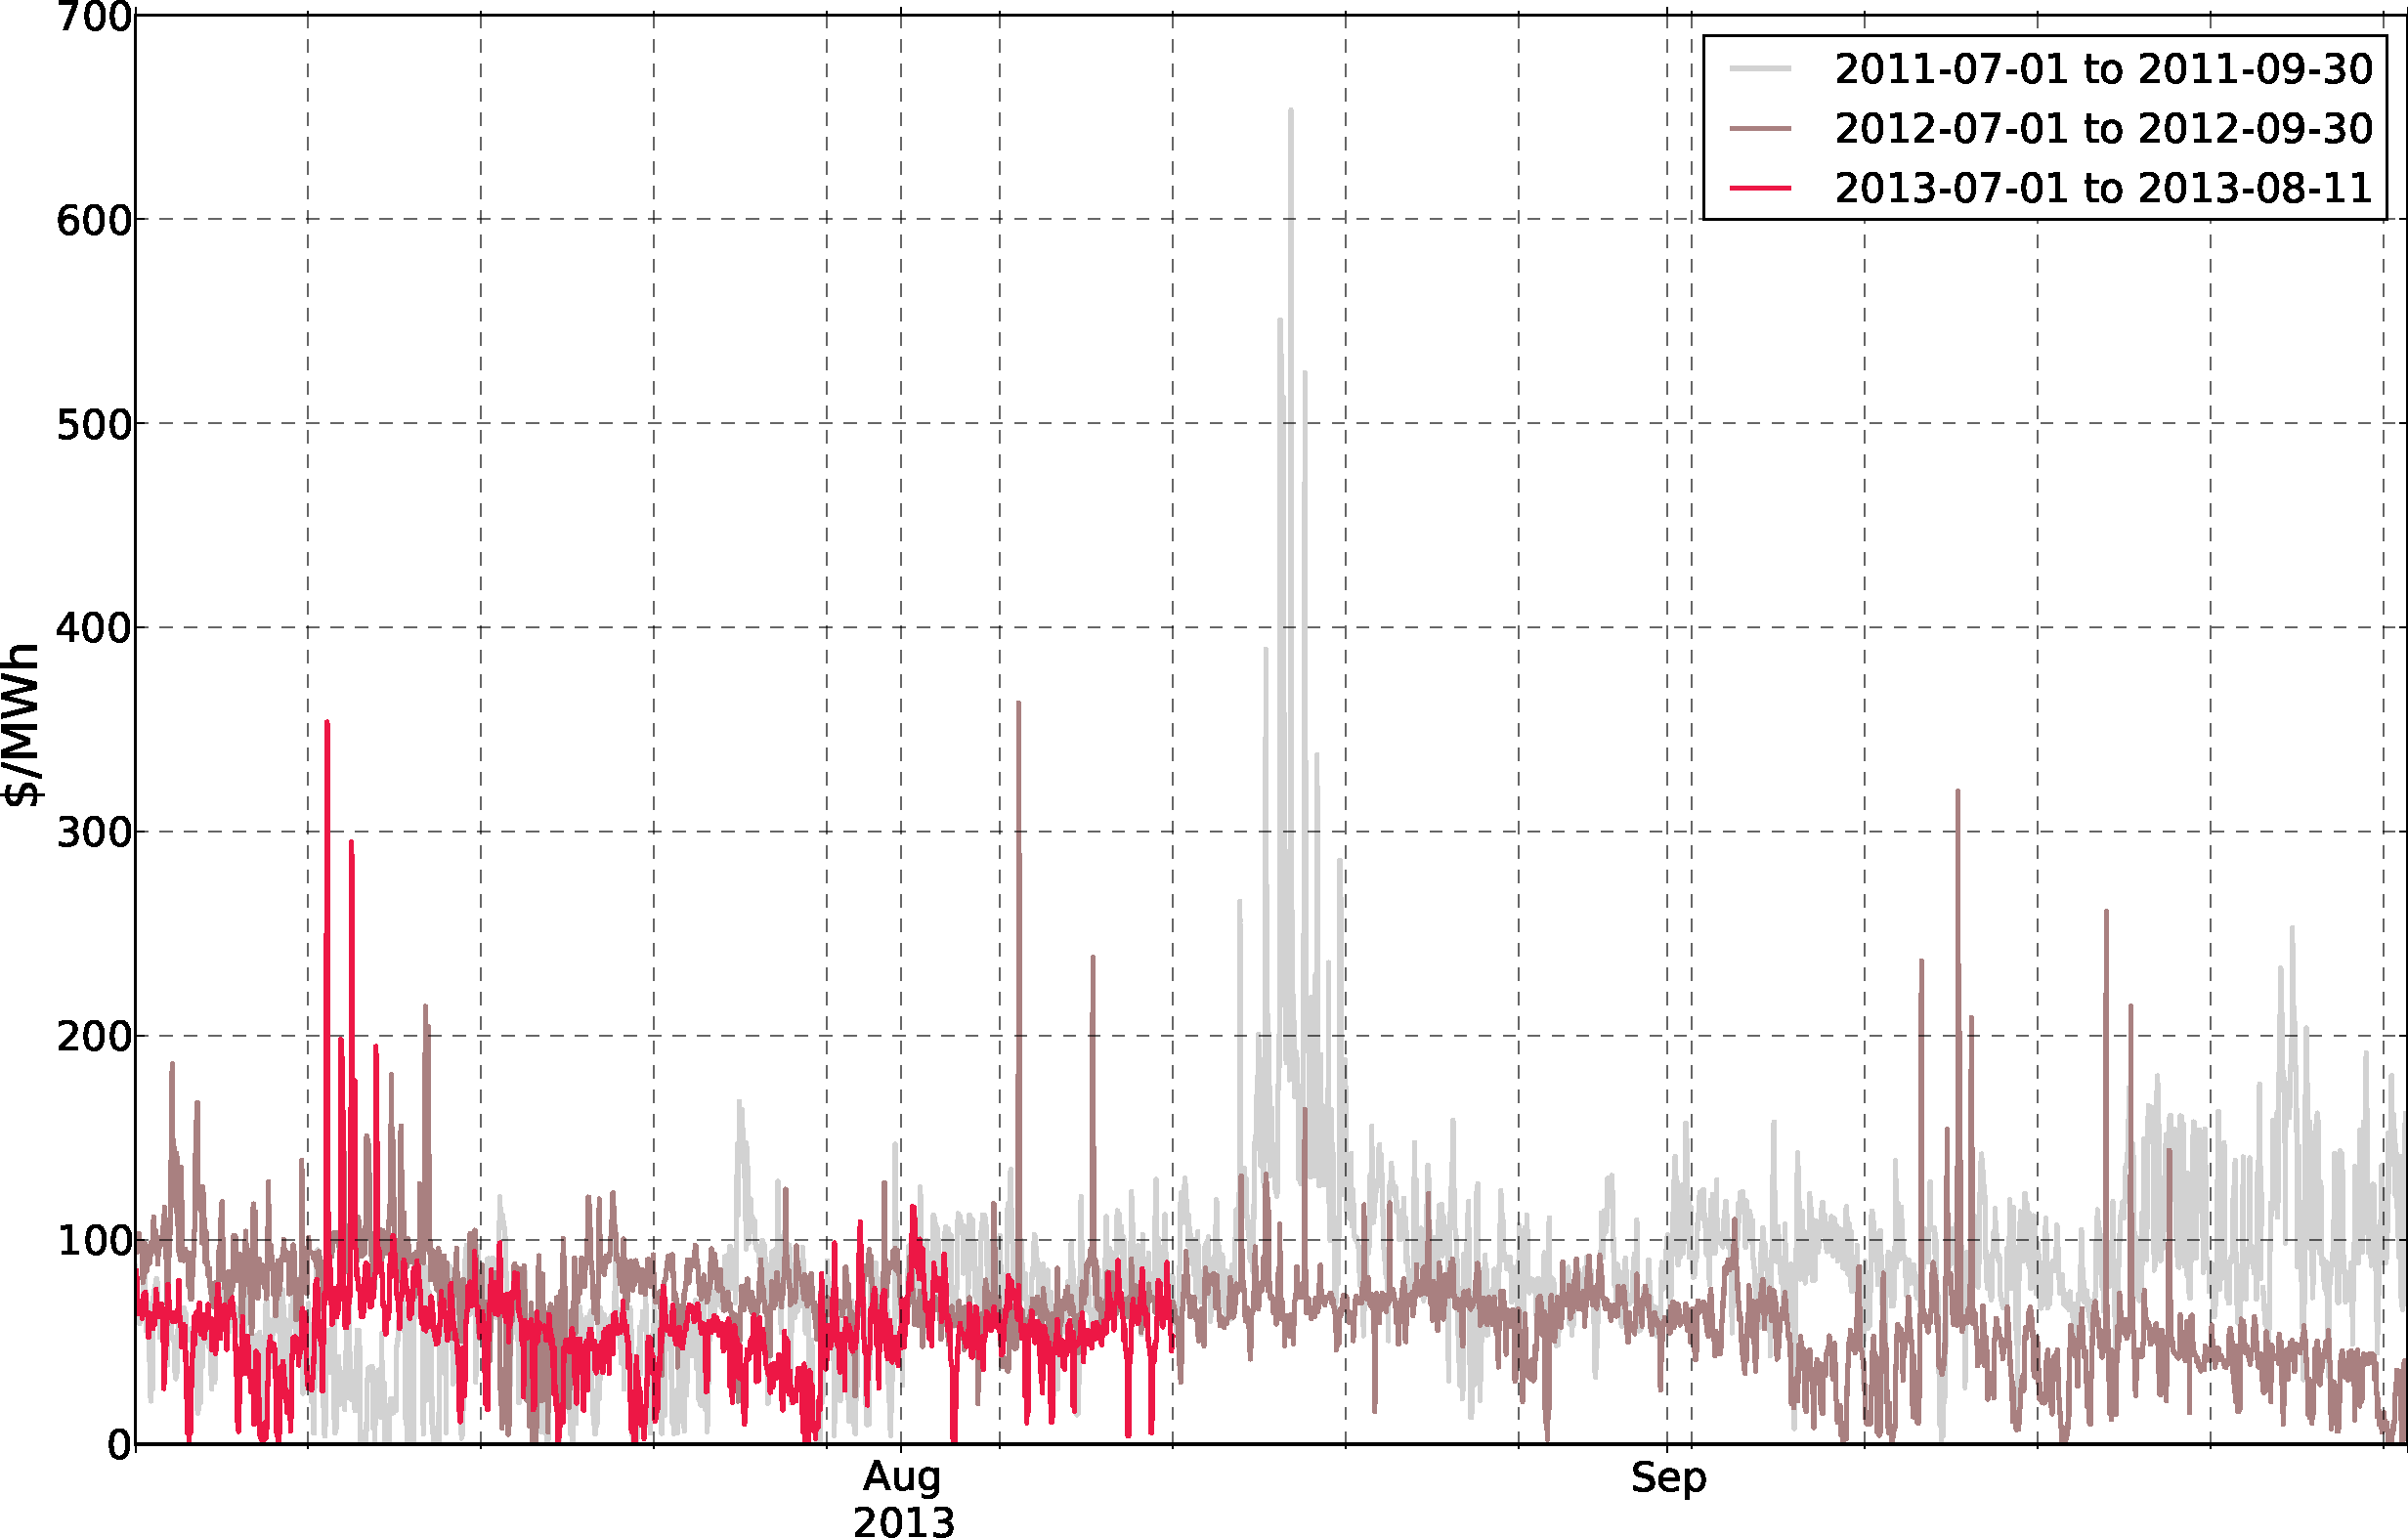
\includegraphics[max size={0.95\textwidth}{0.9\textheight}]{/home/dave/python/reporting/figures/lwap.pdf}
\end{center}
\scriptsize Source: Electricity Authority

\newpage
\section{Hedge Market}

\subsection{Forward Price Curve -- Otahuhu}

\begin{center}
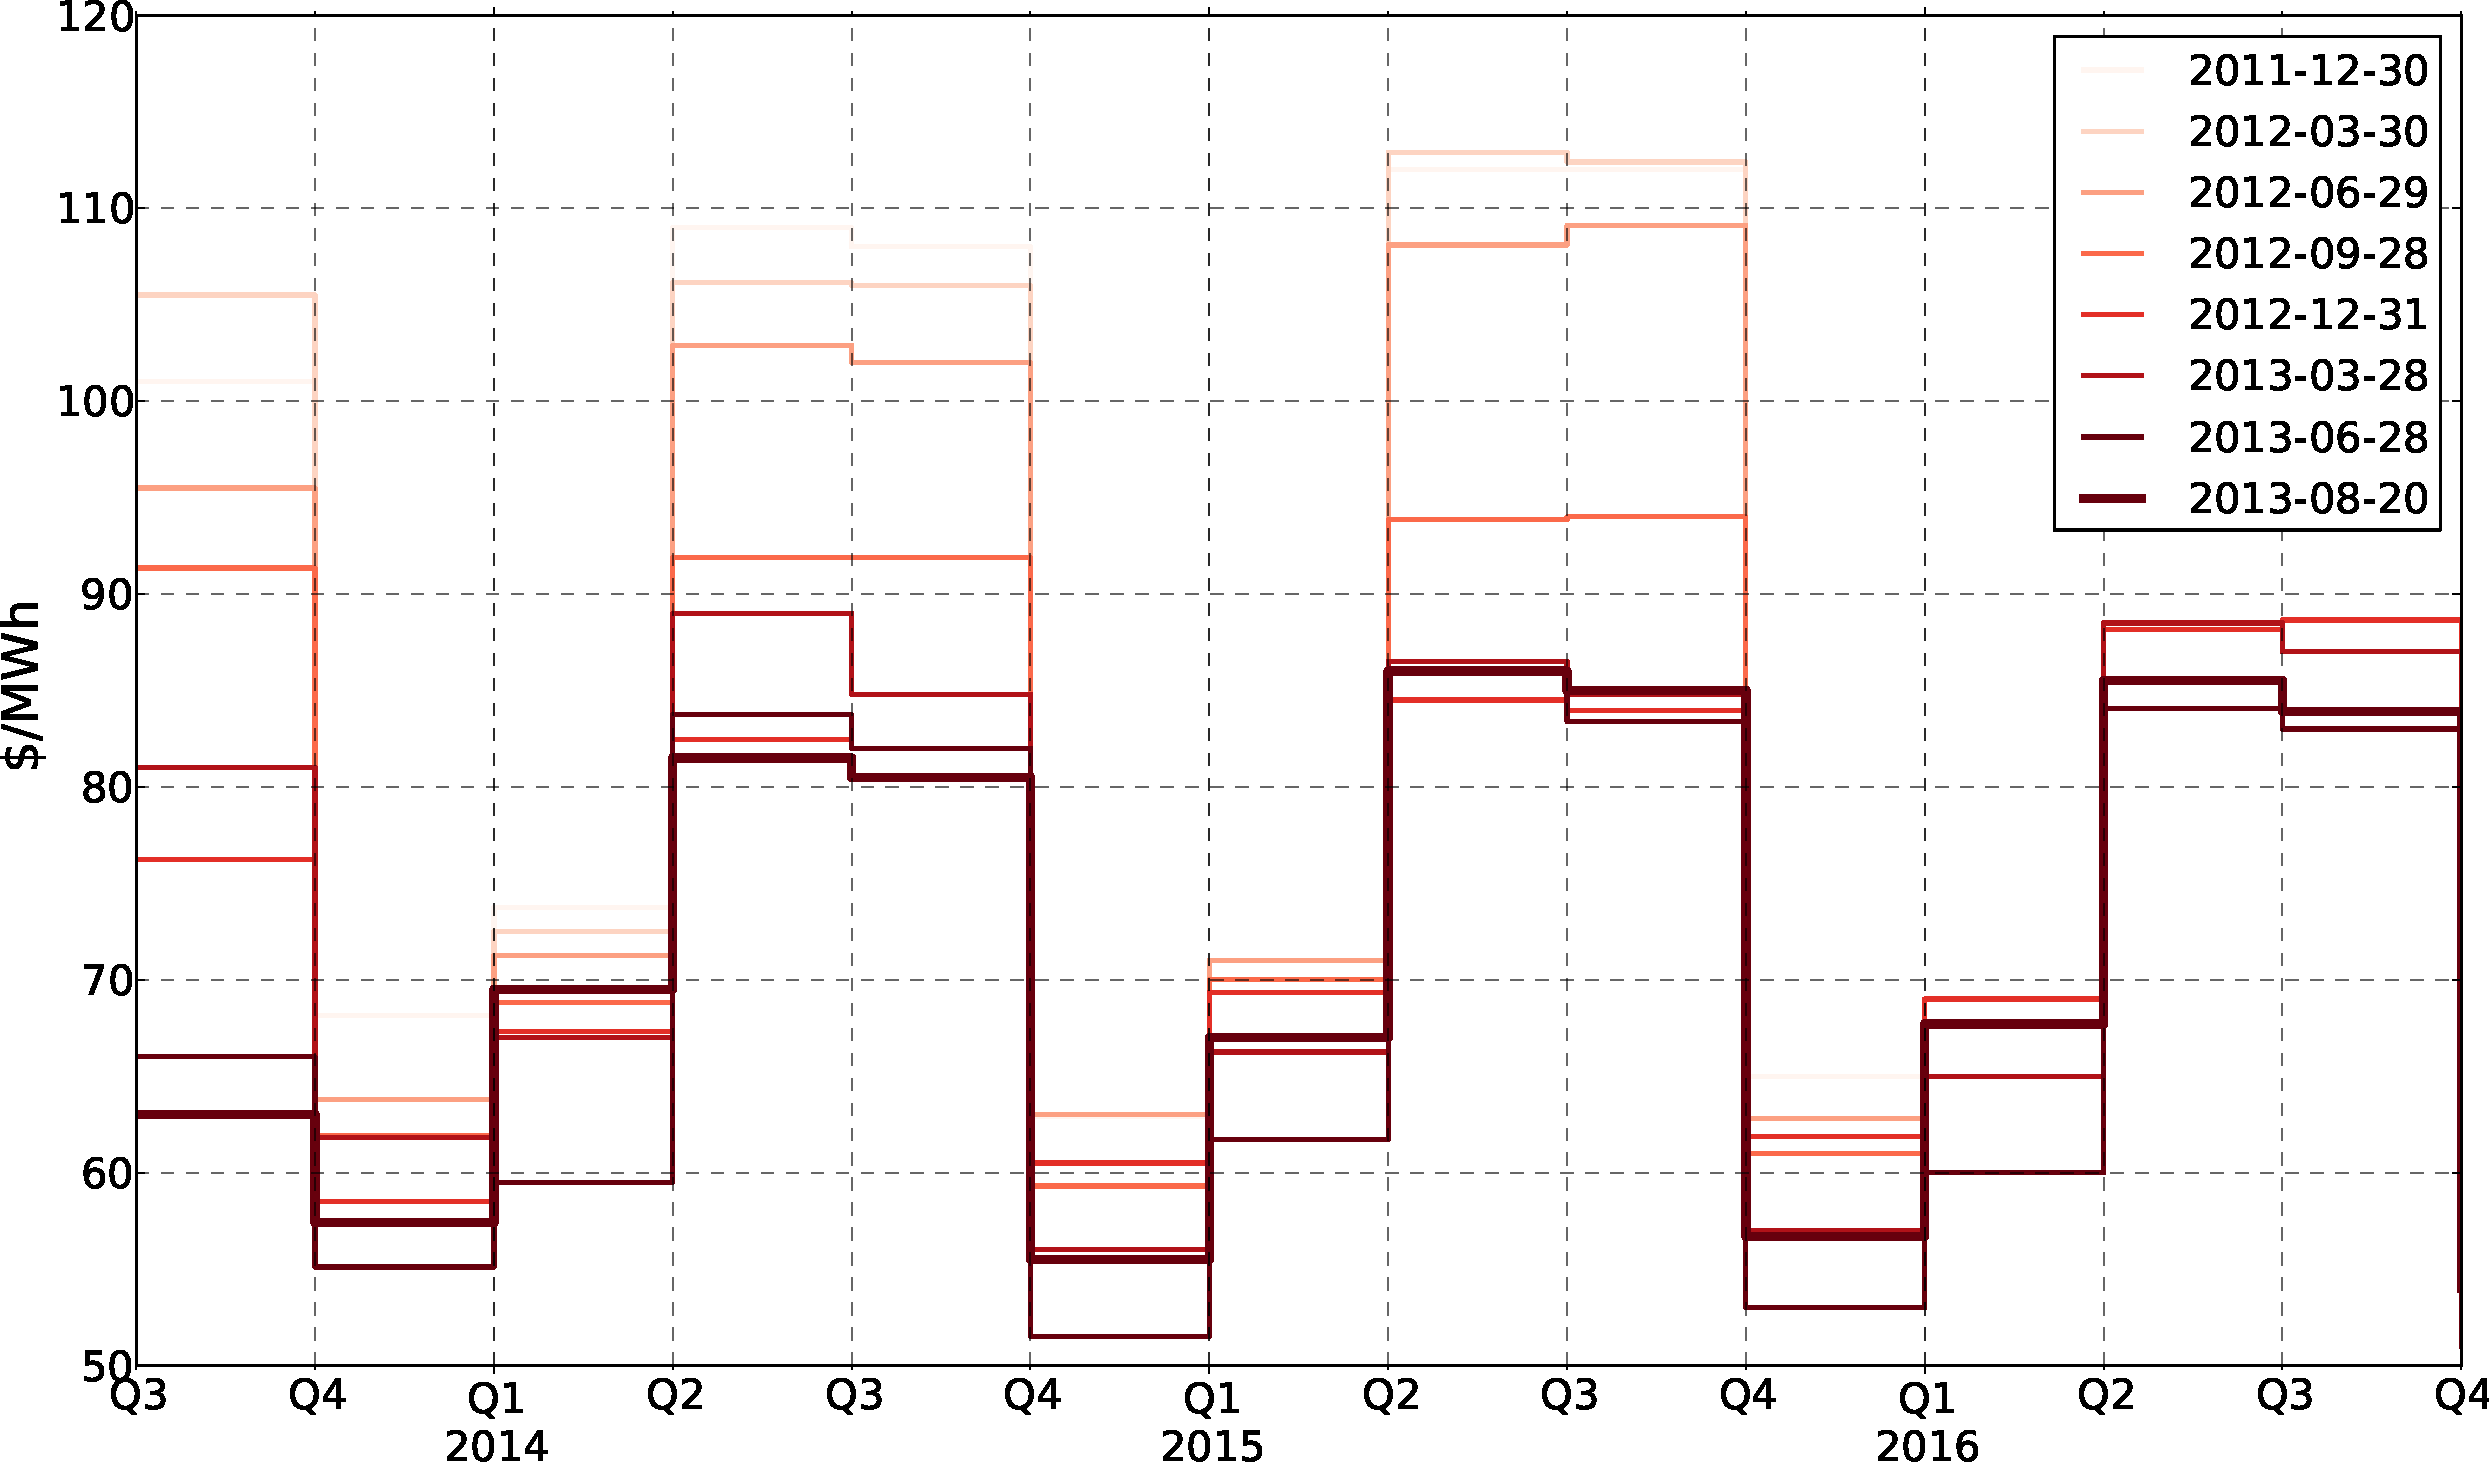
\includegraphics[max size={0.95\textwidth}{0.9\textheight}]{/home/dave/python/reporting/figures/ota_fpc.pdf}
\end{center}
\scriptsize Source: ASX \url{http://www.asx.com.au}

\subsection{Forward Price Curve -- Benmore}

\begin{center}
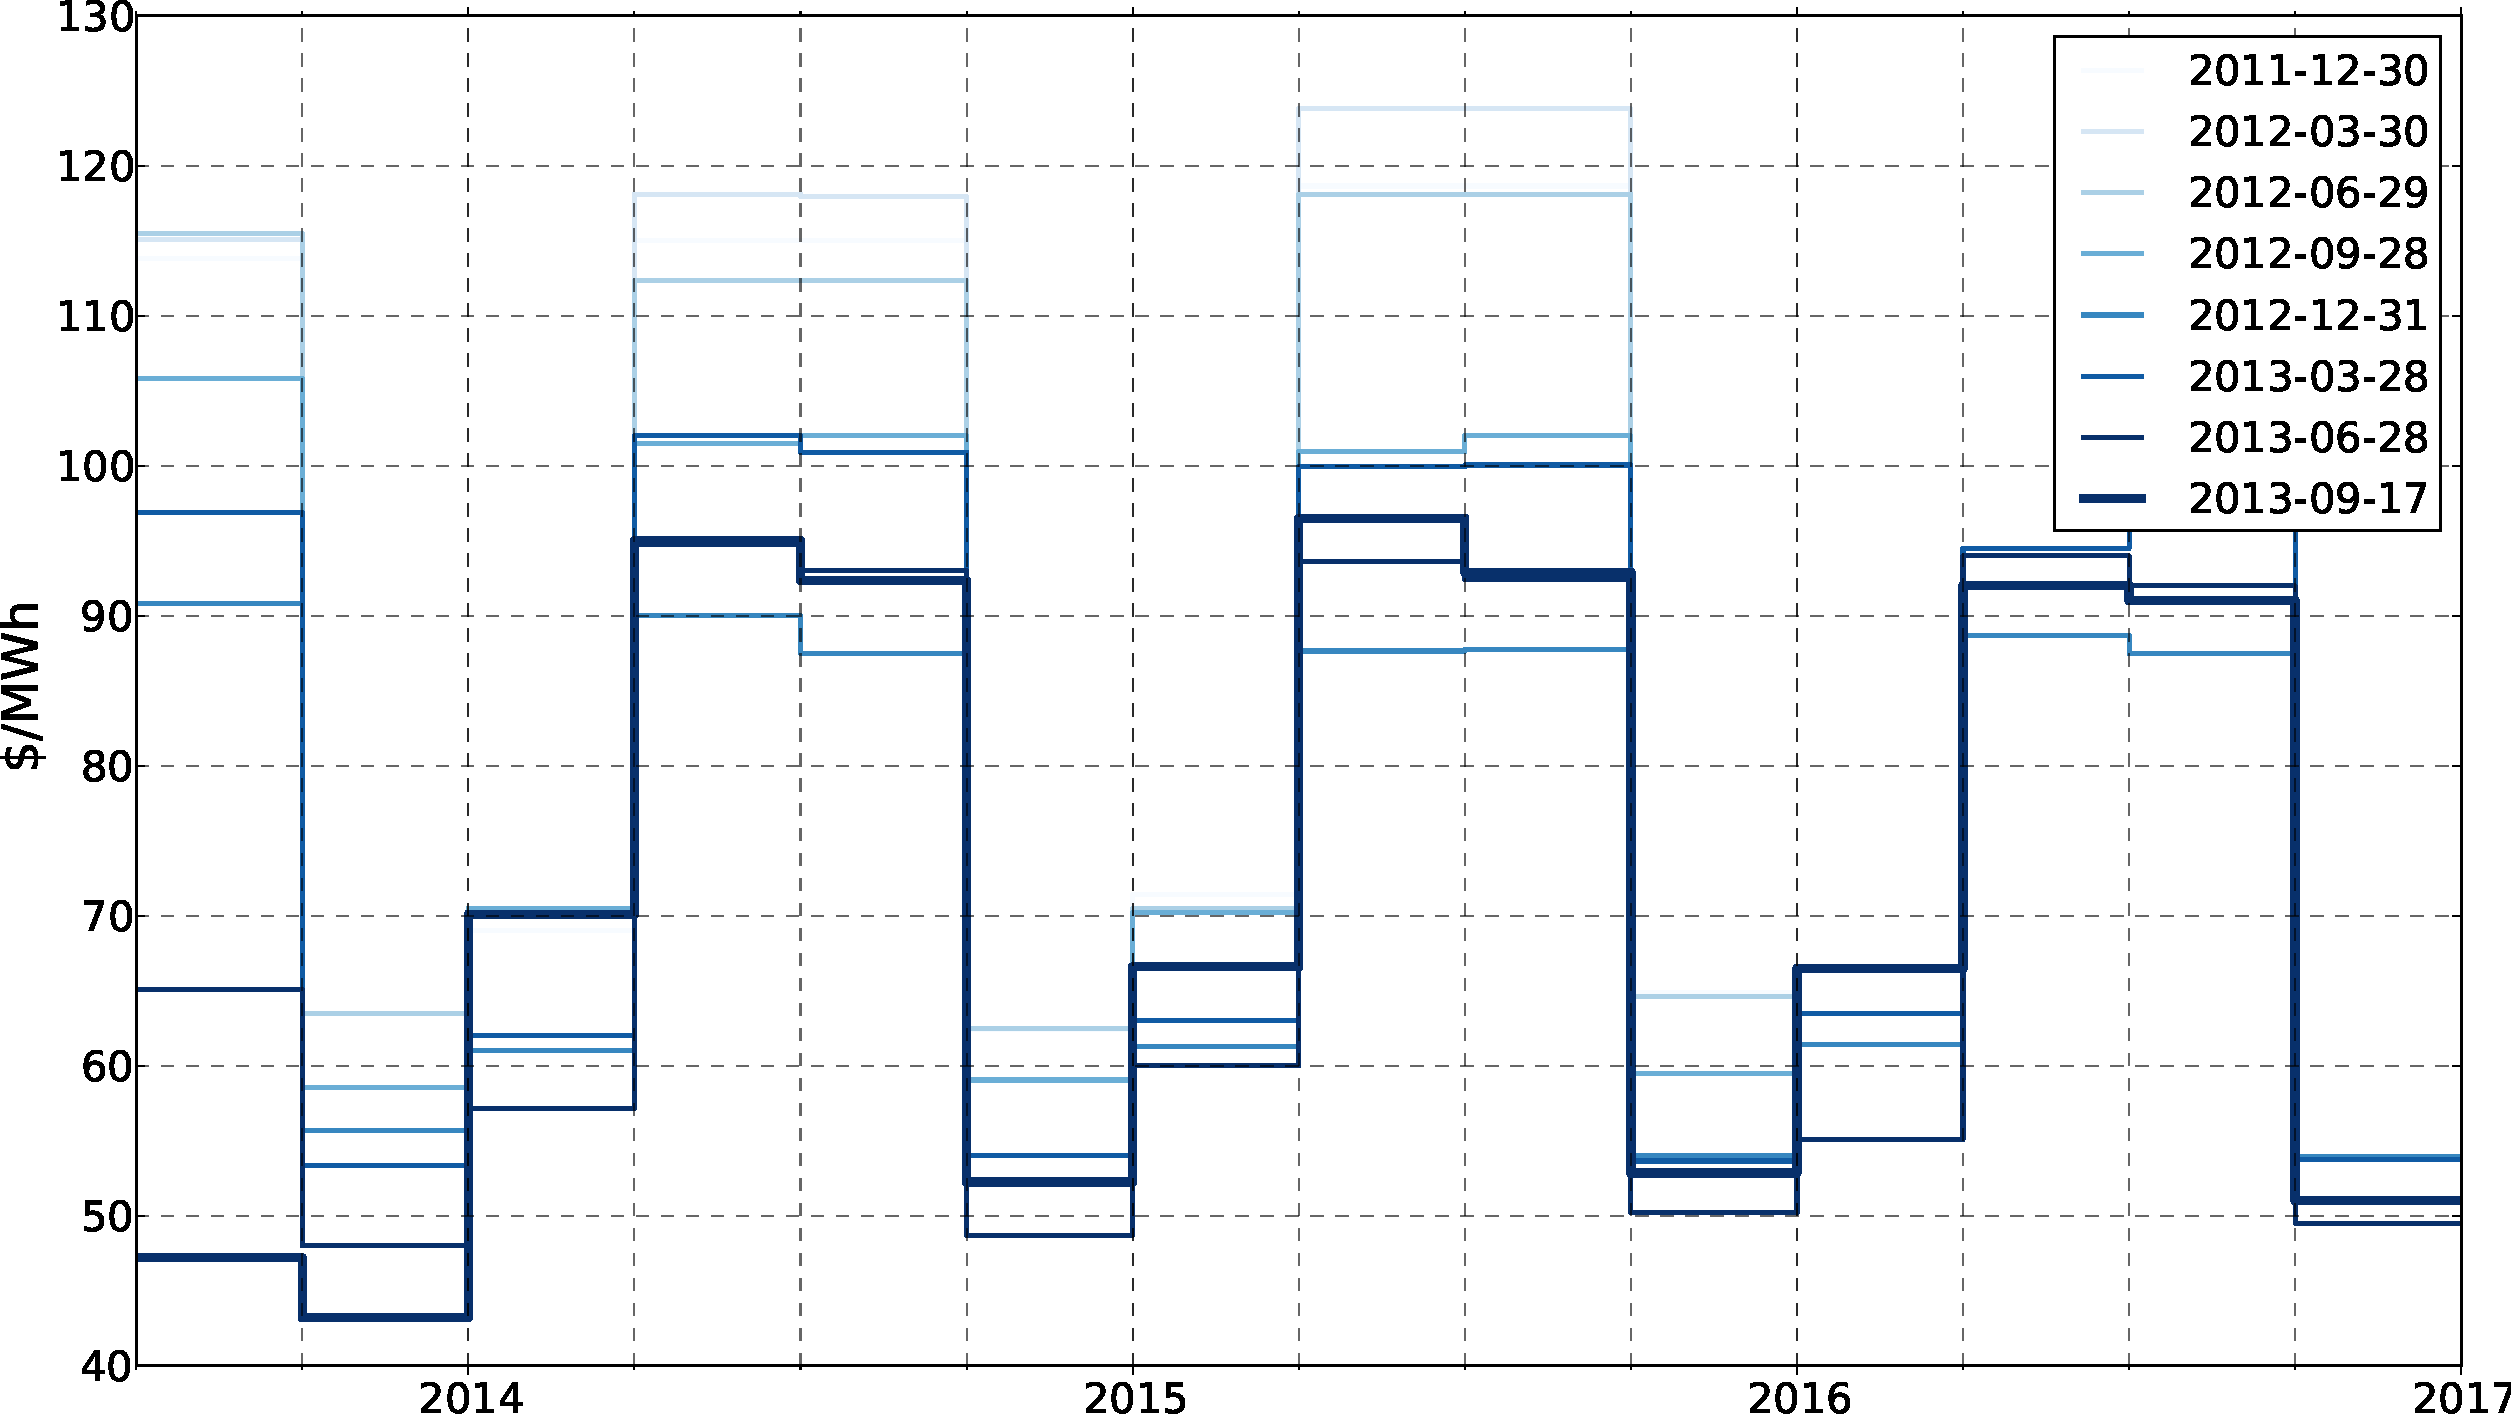
\includegraphics[max size={0.95\textwidth}{0.9\textheight}]{/home/dave/python/reporting/figures/ben_fpc.pdf}
\end{center}
\scriptsize Source: ASX \url{http://www.asx.com.au}

\subsection{Current quarter trends}

\begin{center}
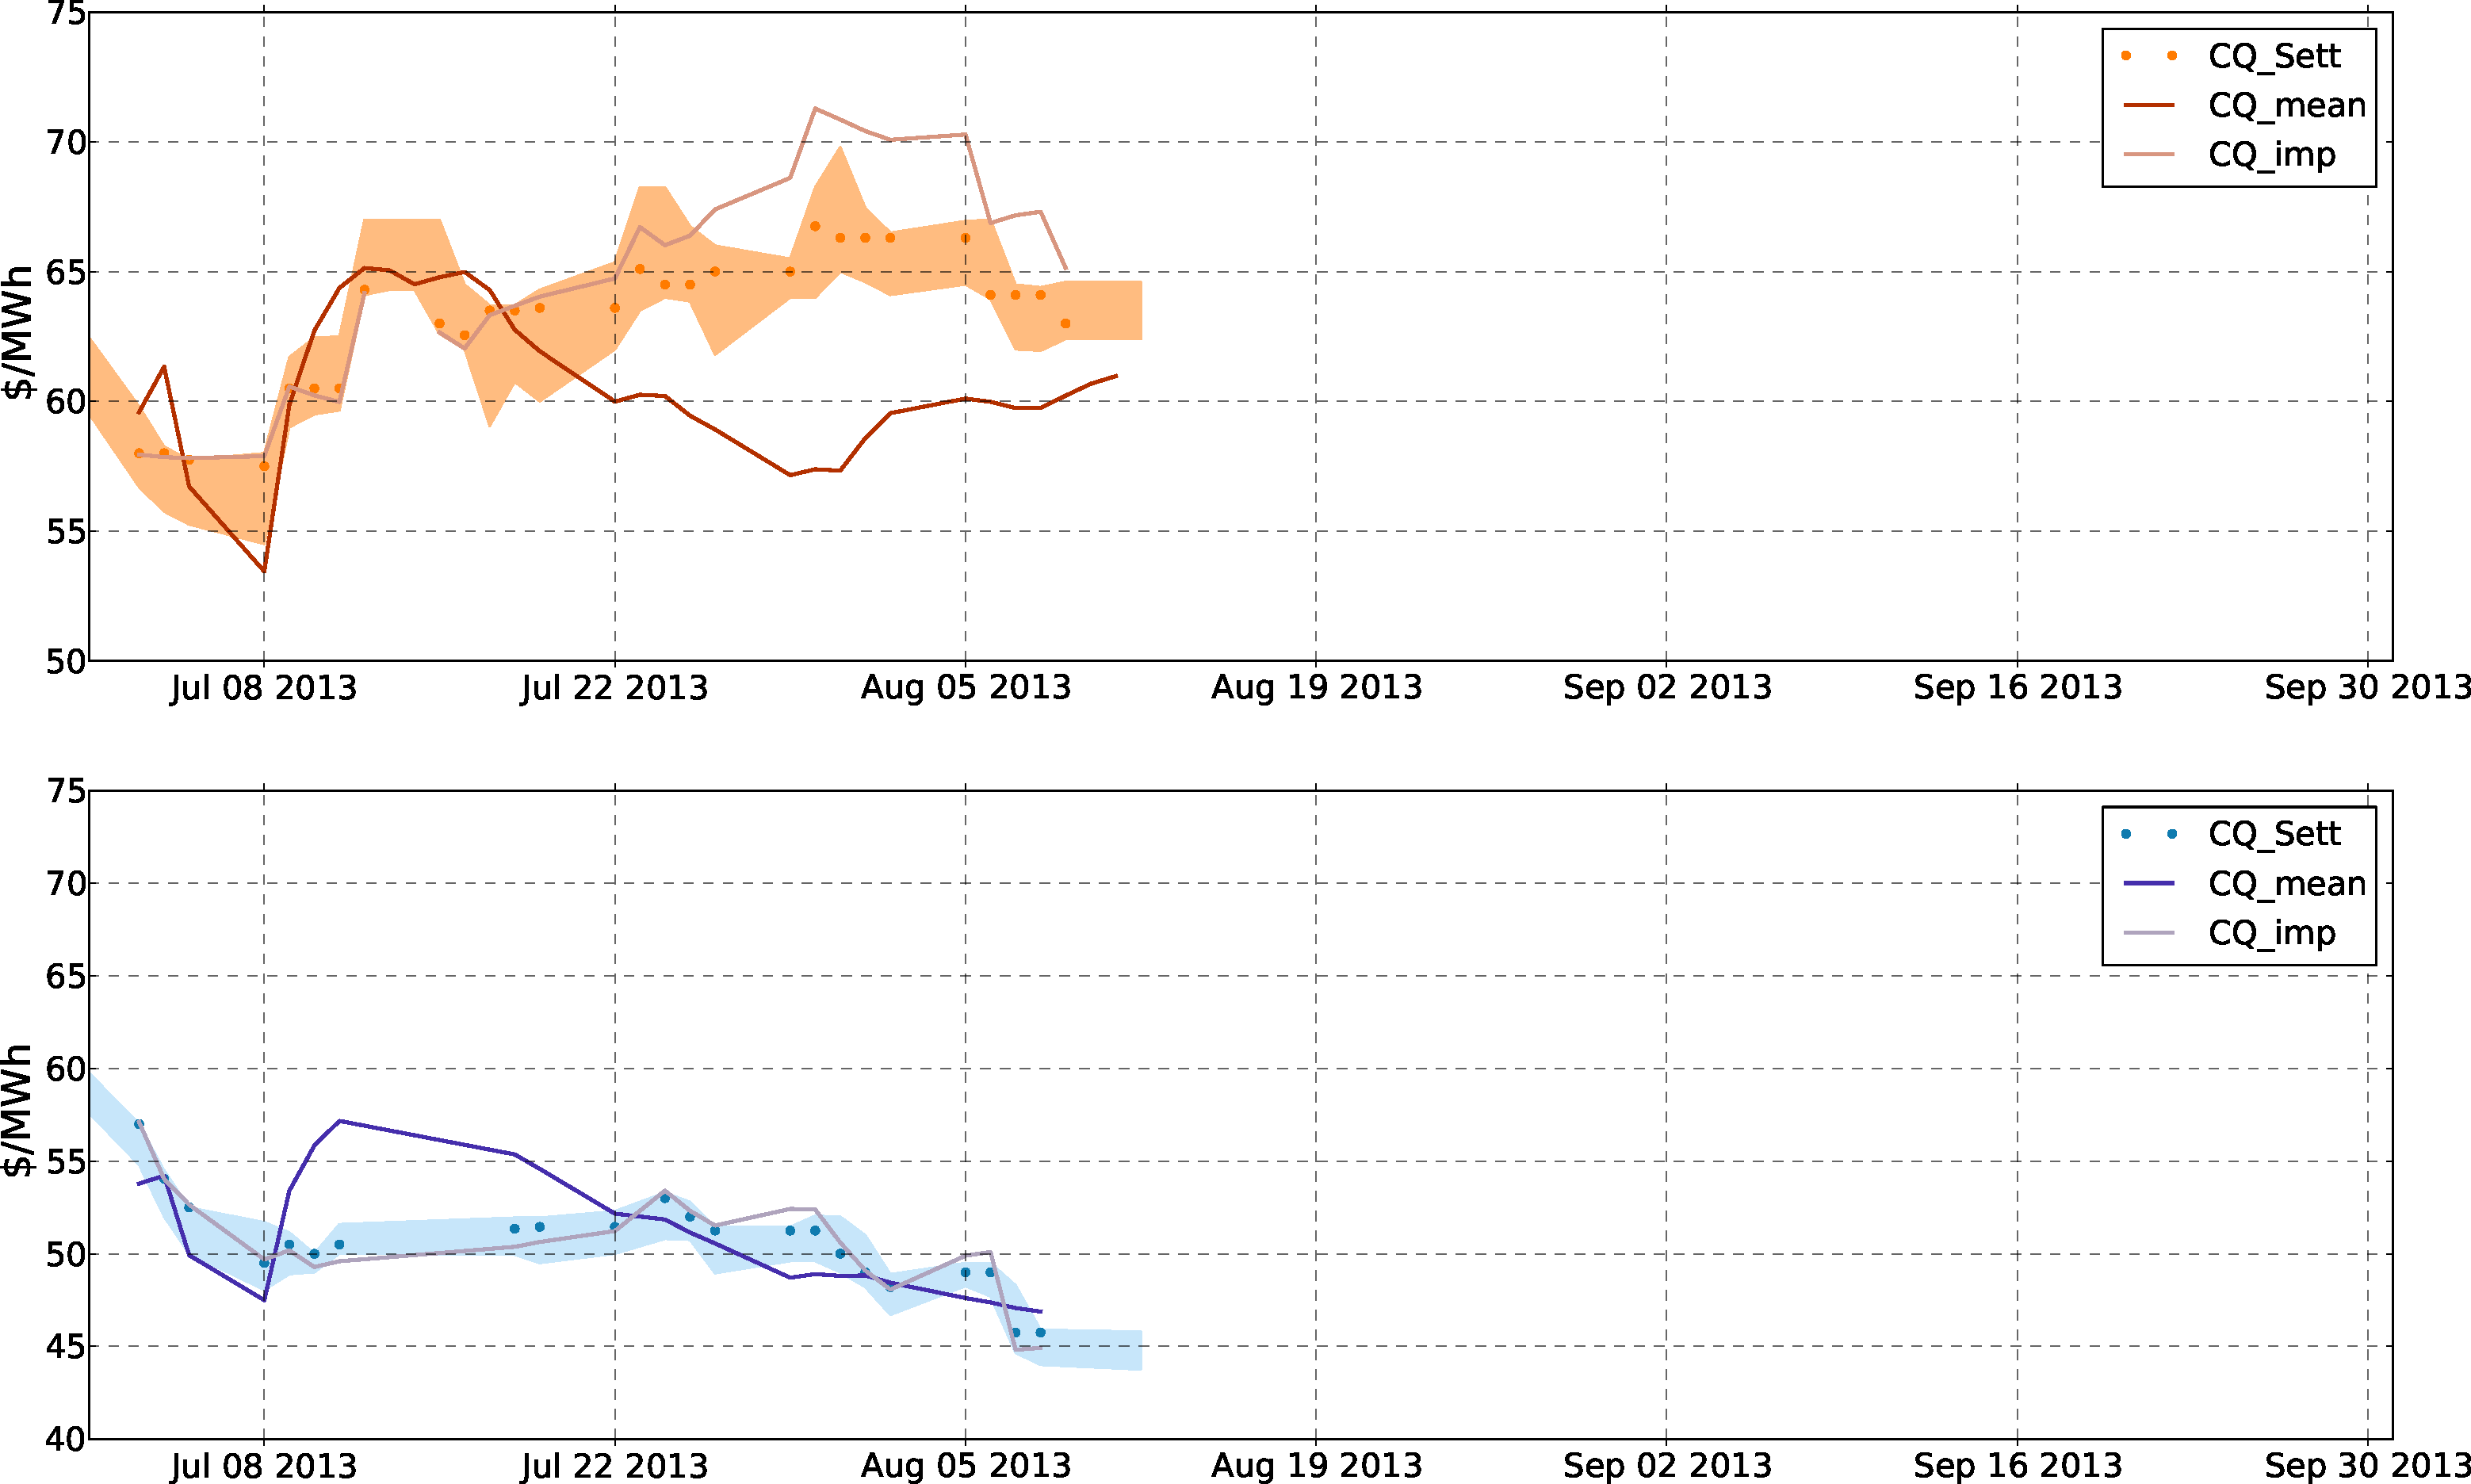
\includegraphics[max size={\textwidth}{0.9\textheight}]{/home/dave/python/reporting/figures/cq_trend.pdf}
\end{center}
\scriptsize Note: The implied spot price is the calculated average spot price over the remainder of the quarter, implied by the current settlement price.

\scriptsize Source: ASX \url{http://www.asx.com.au}

\subsection{Monthly Volumes}

\begin{center}
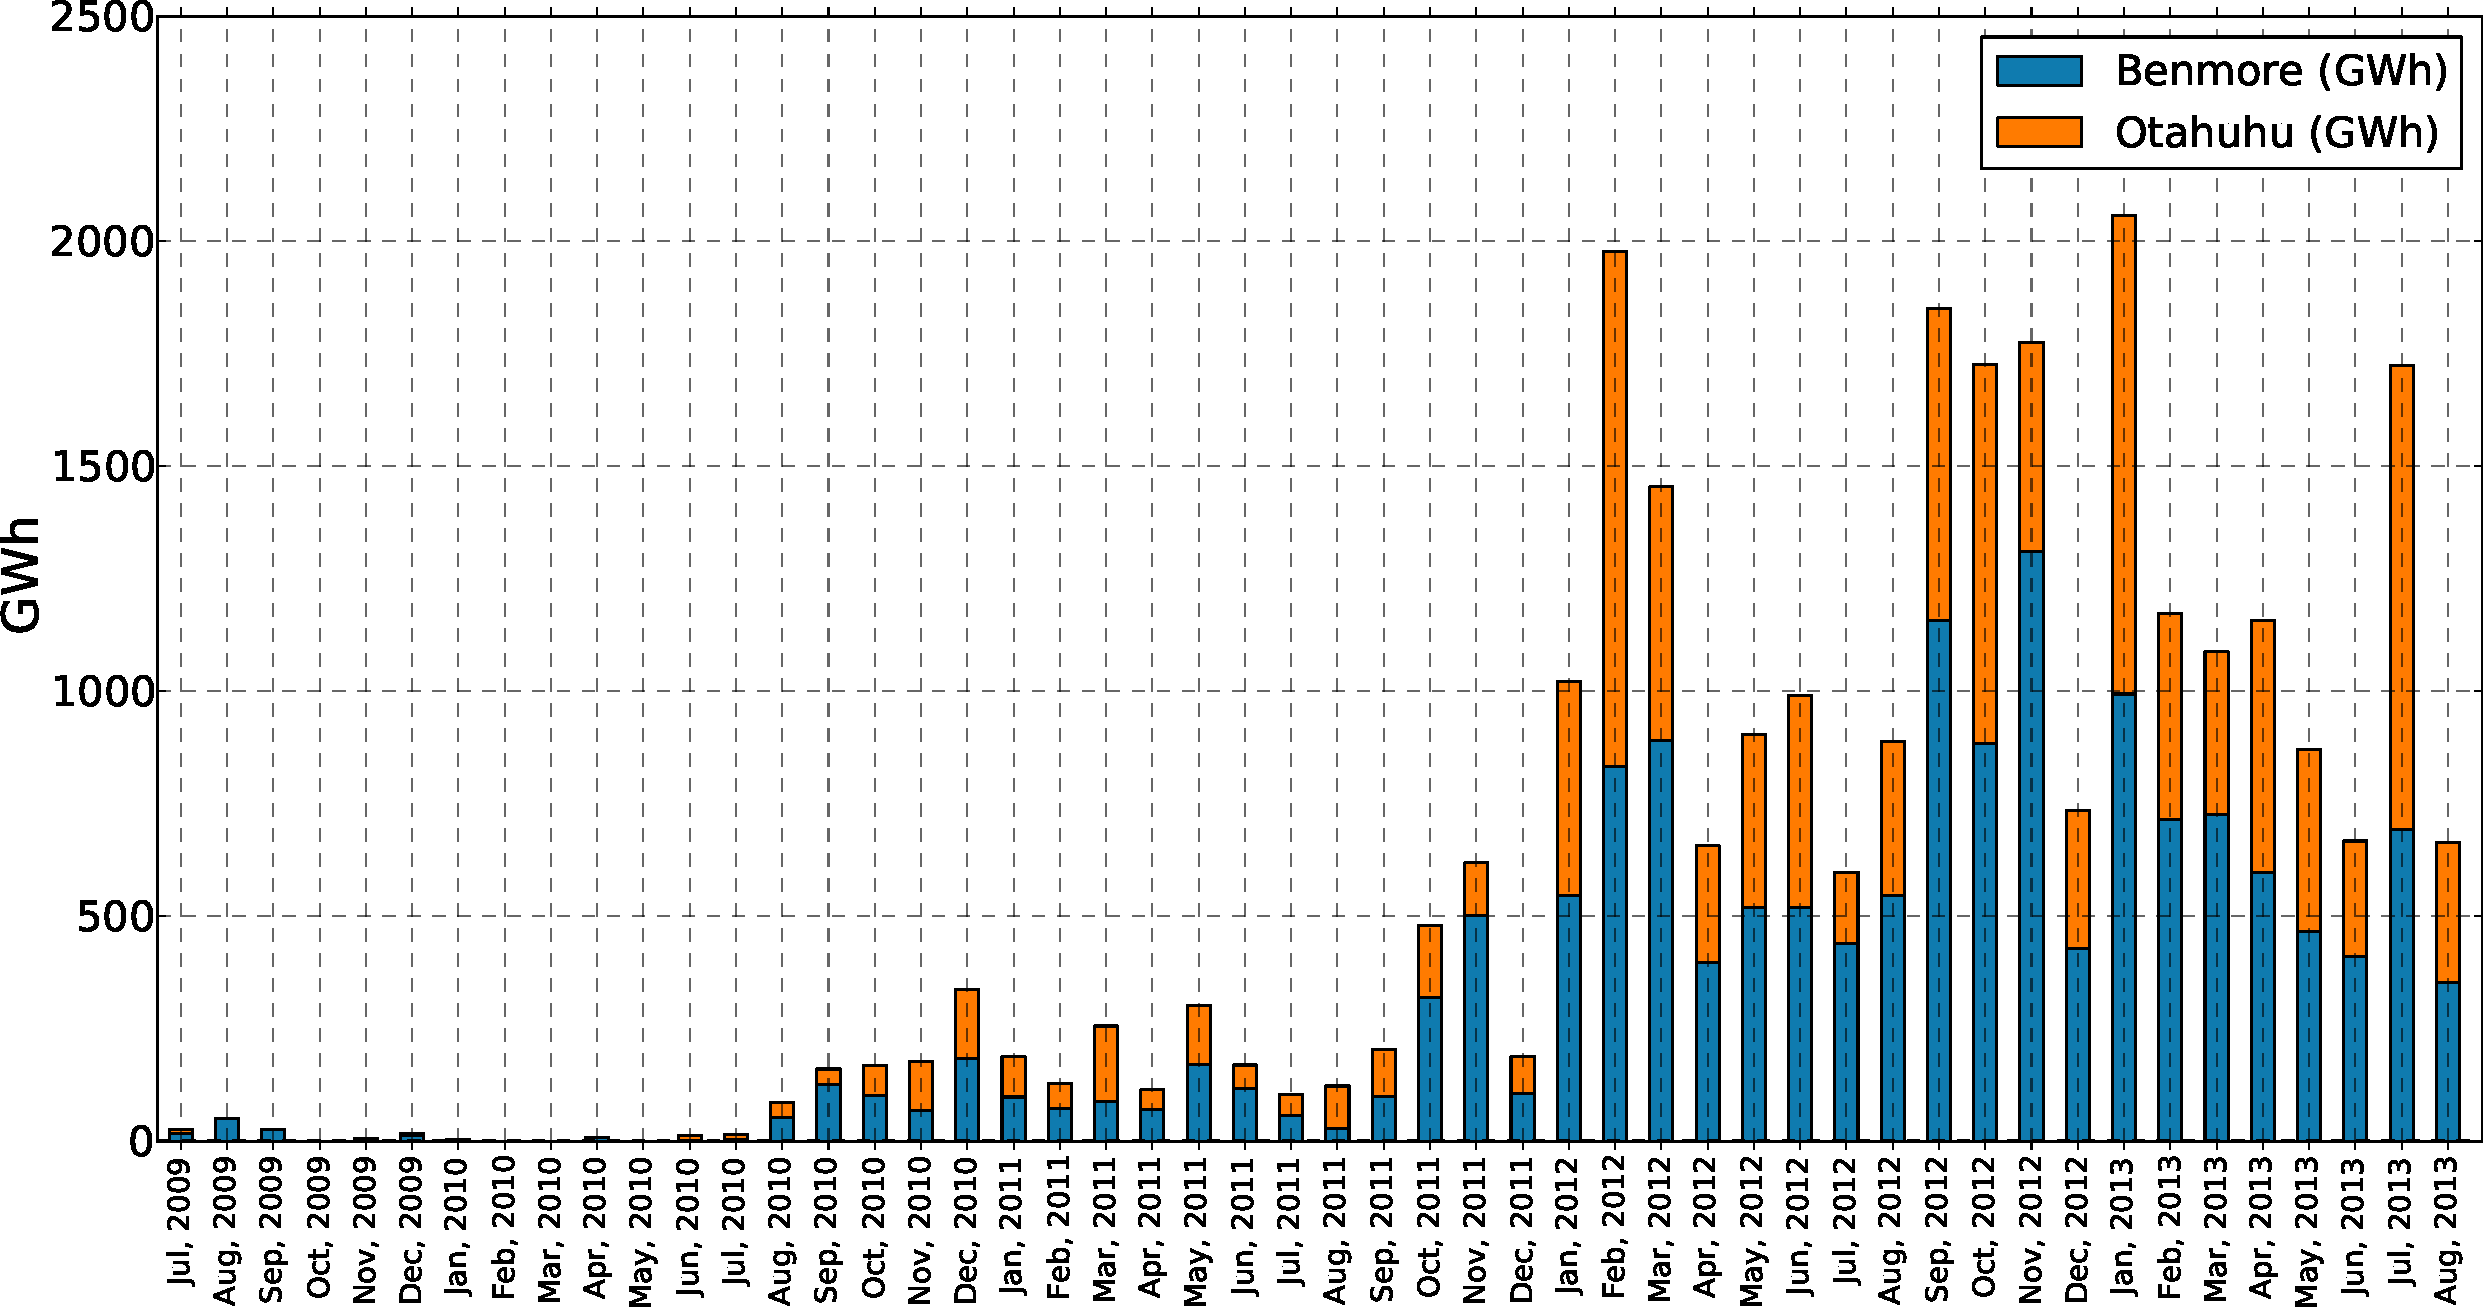
\includegraphics[max size={\textwidth}{0.9\textheight}]{/home/dave/python/reporting/figures/asx_volumes.pdf}
\end{center}
\scriptsize Source: ASX \url{http://www.asx.com.au}

\subsection{Open Interest}
\vspace{2cm}
\begin{center}
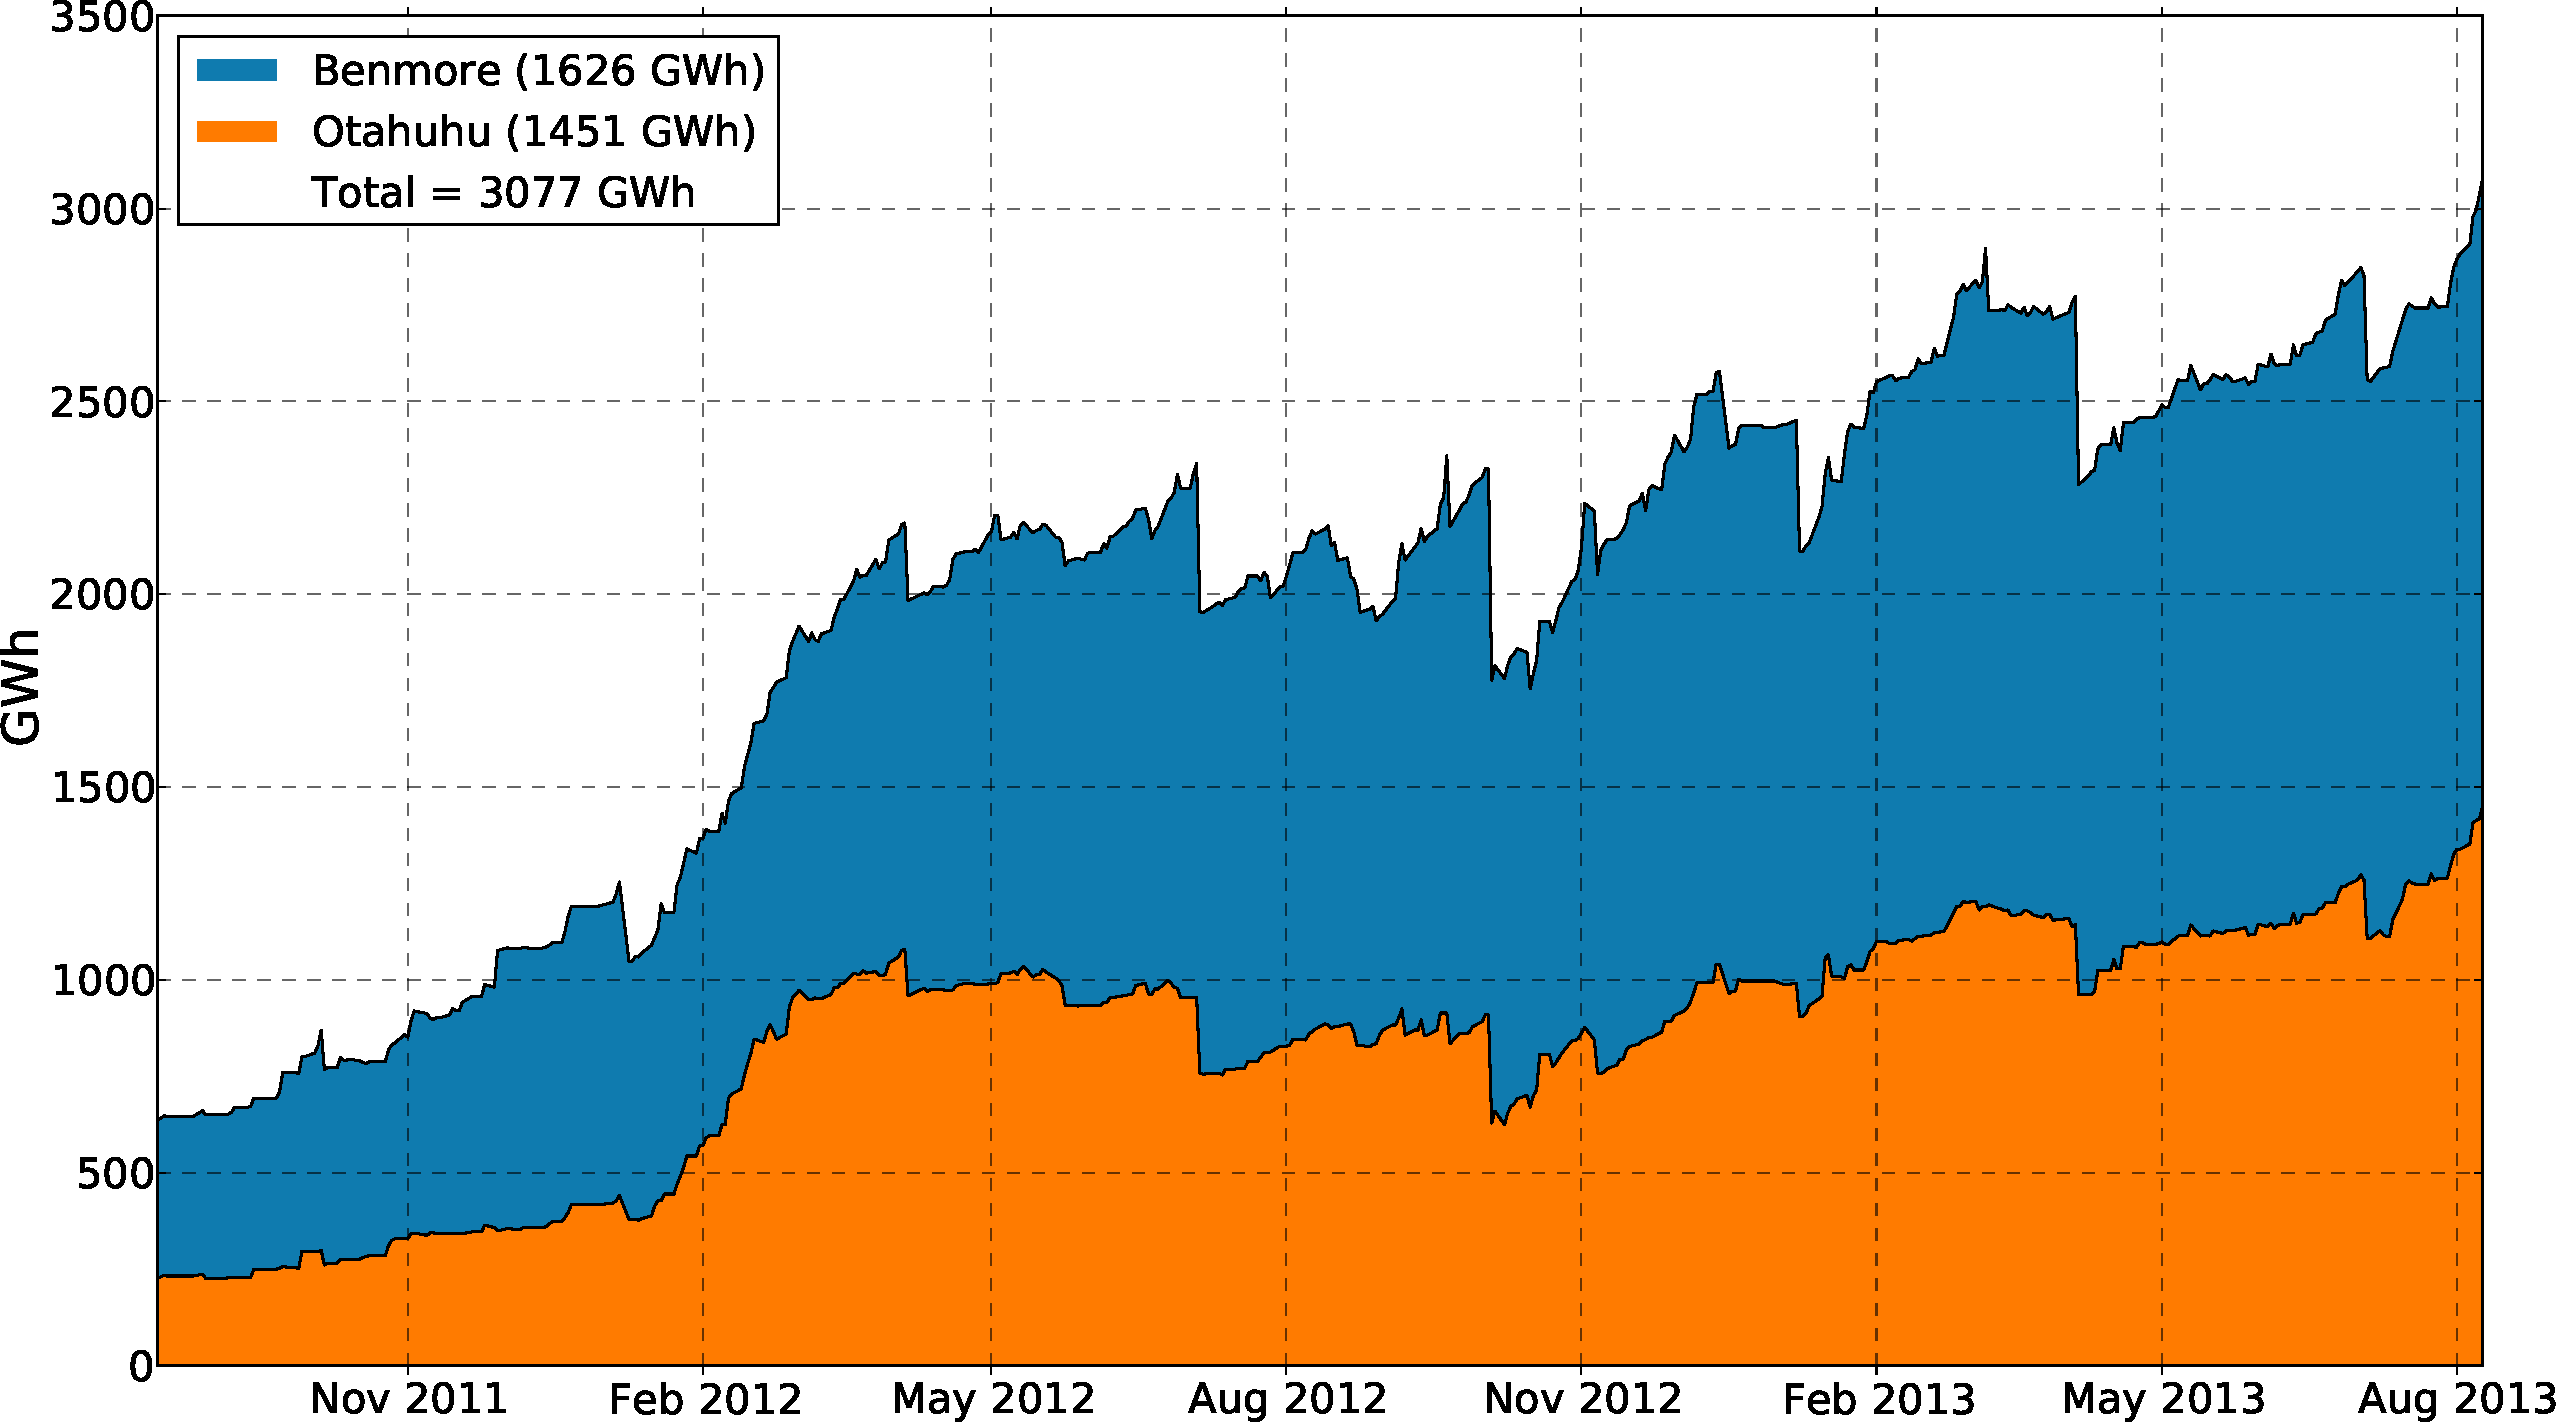
\includegraphics[max size={\textwidth}{0.9\textheight}]{/home/dave/python/reporting/figures/asx_opint.pdf}
\end{center}
\scriptsize Source: ASX \url{http://www.asx.com.au}

\subsection{Trends over last year - Otahuhu}

\begin{center}
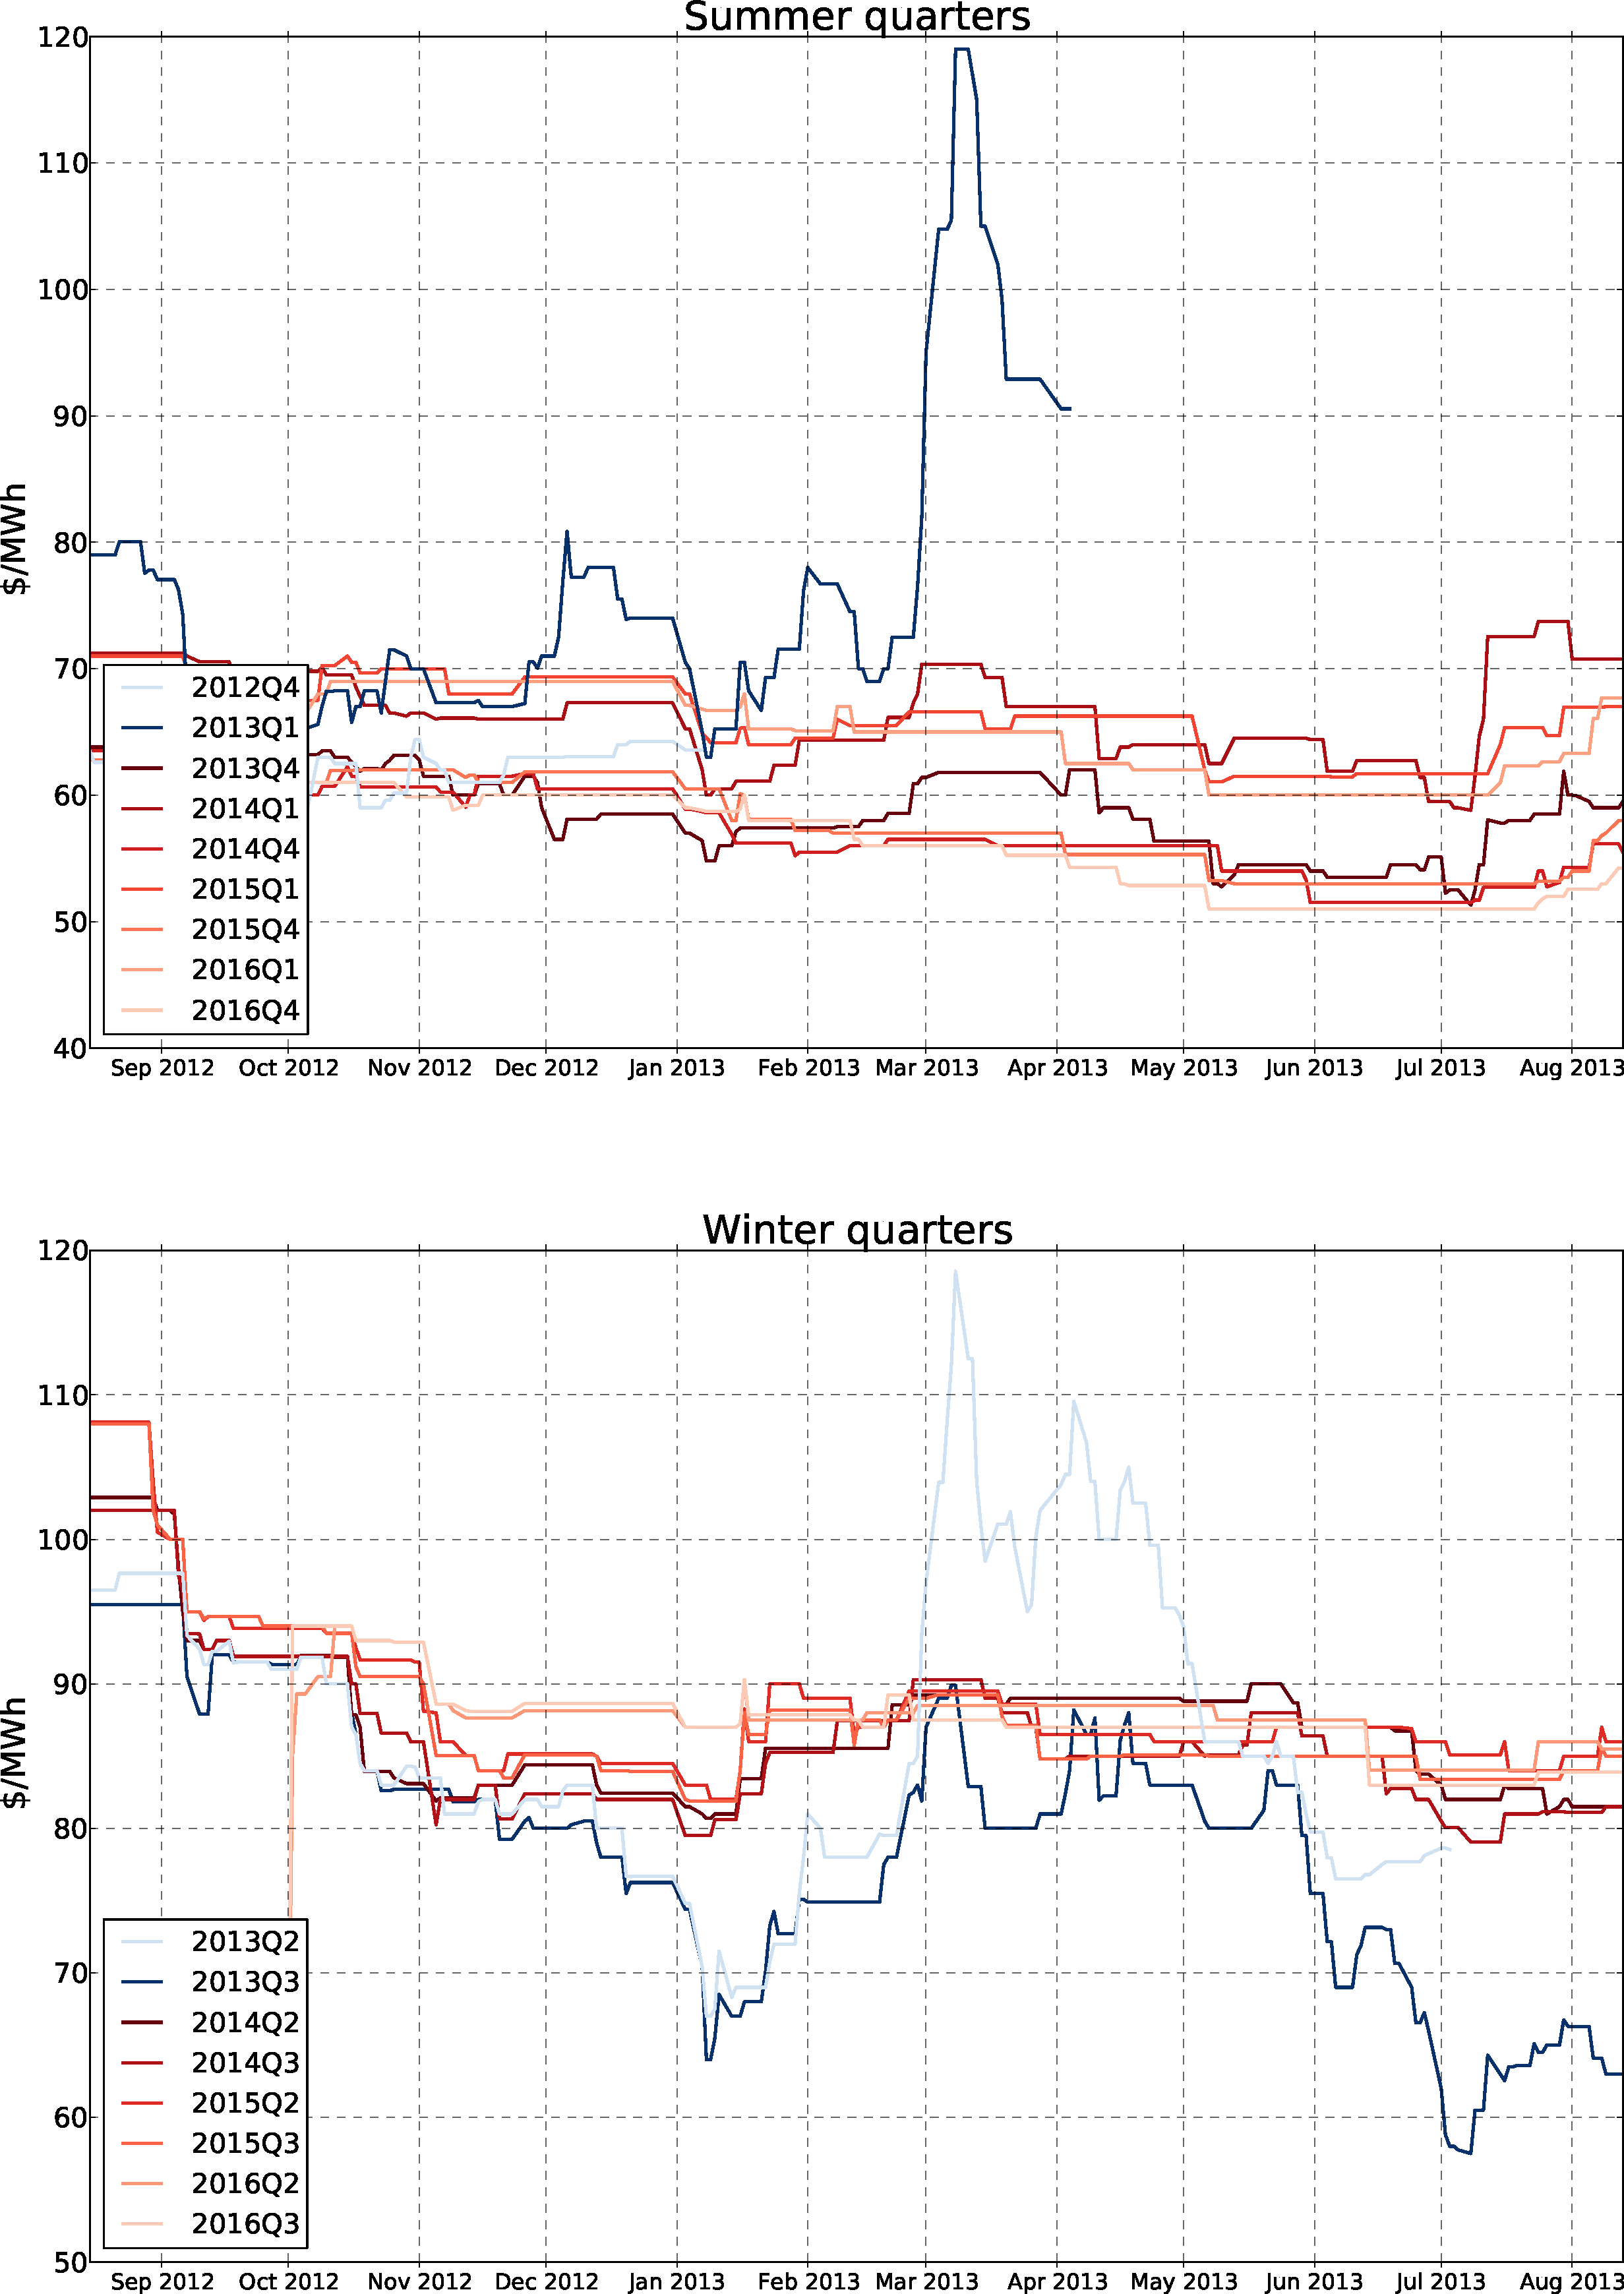
\includegraphics[max size={\textwidth}{0.9\textheight}]{/home/dave/python/reporting/figures/asx_ota_year.pdf}
\end{center}
\scriptsize Source: ASX \url{http://www.asx.com.au}

\subsection{Trends over last year - Benmore}

\begin{center}
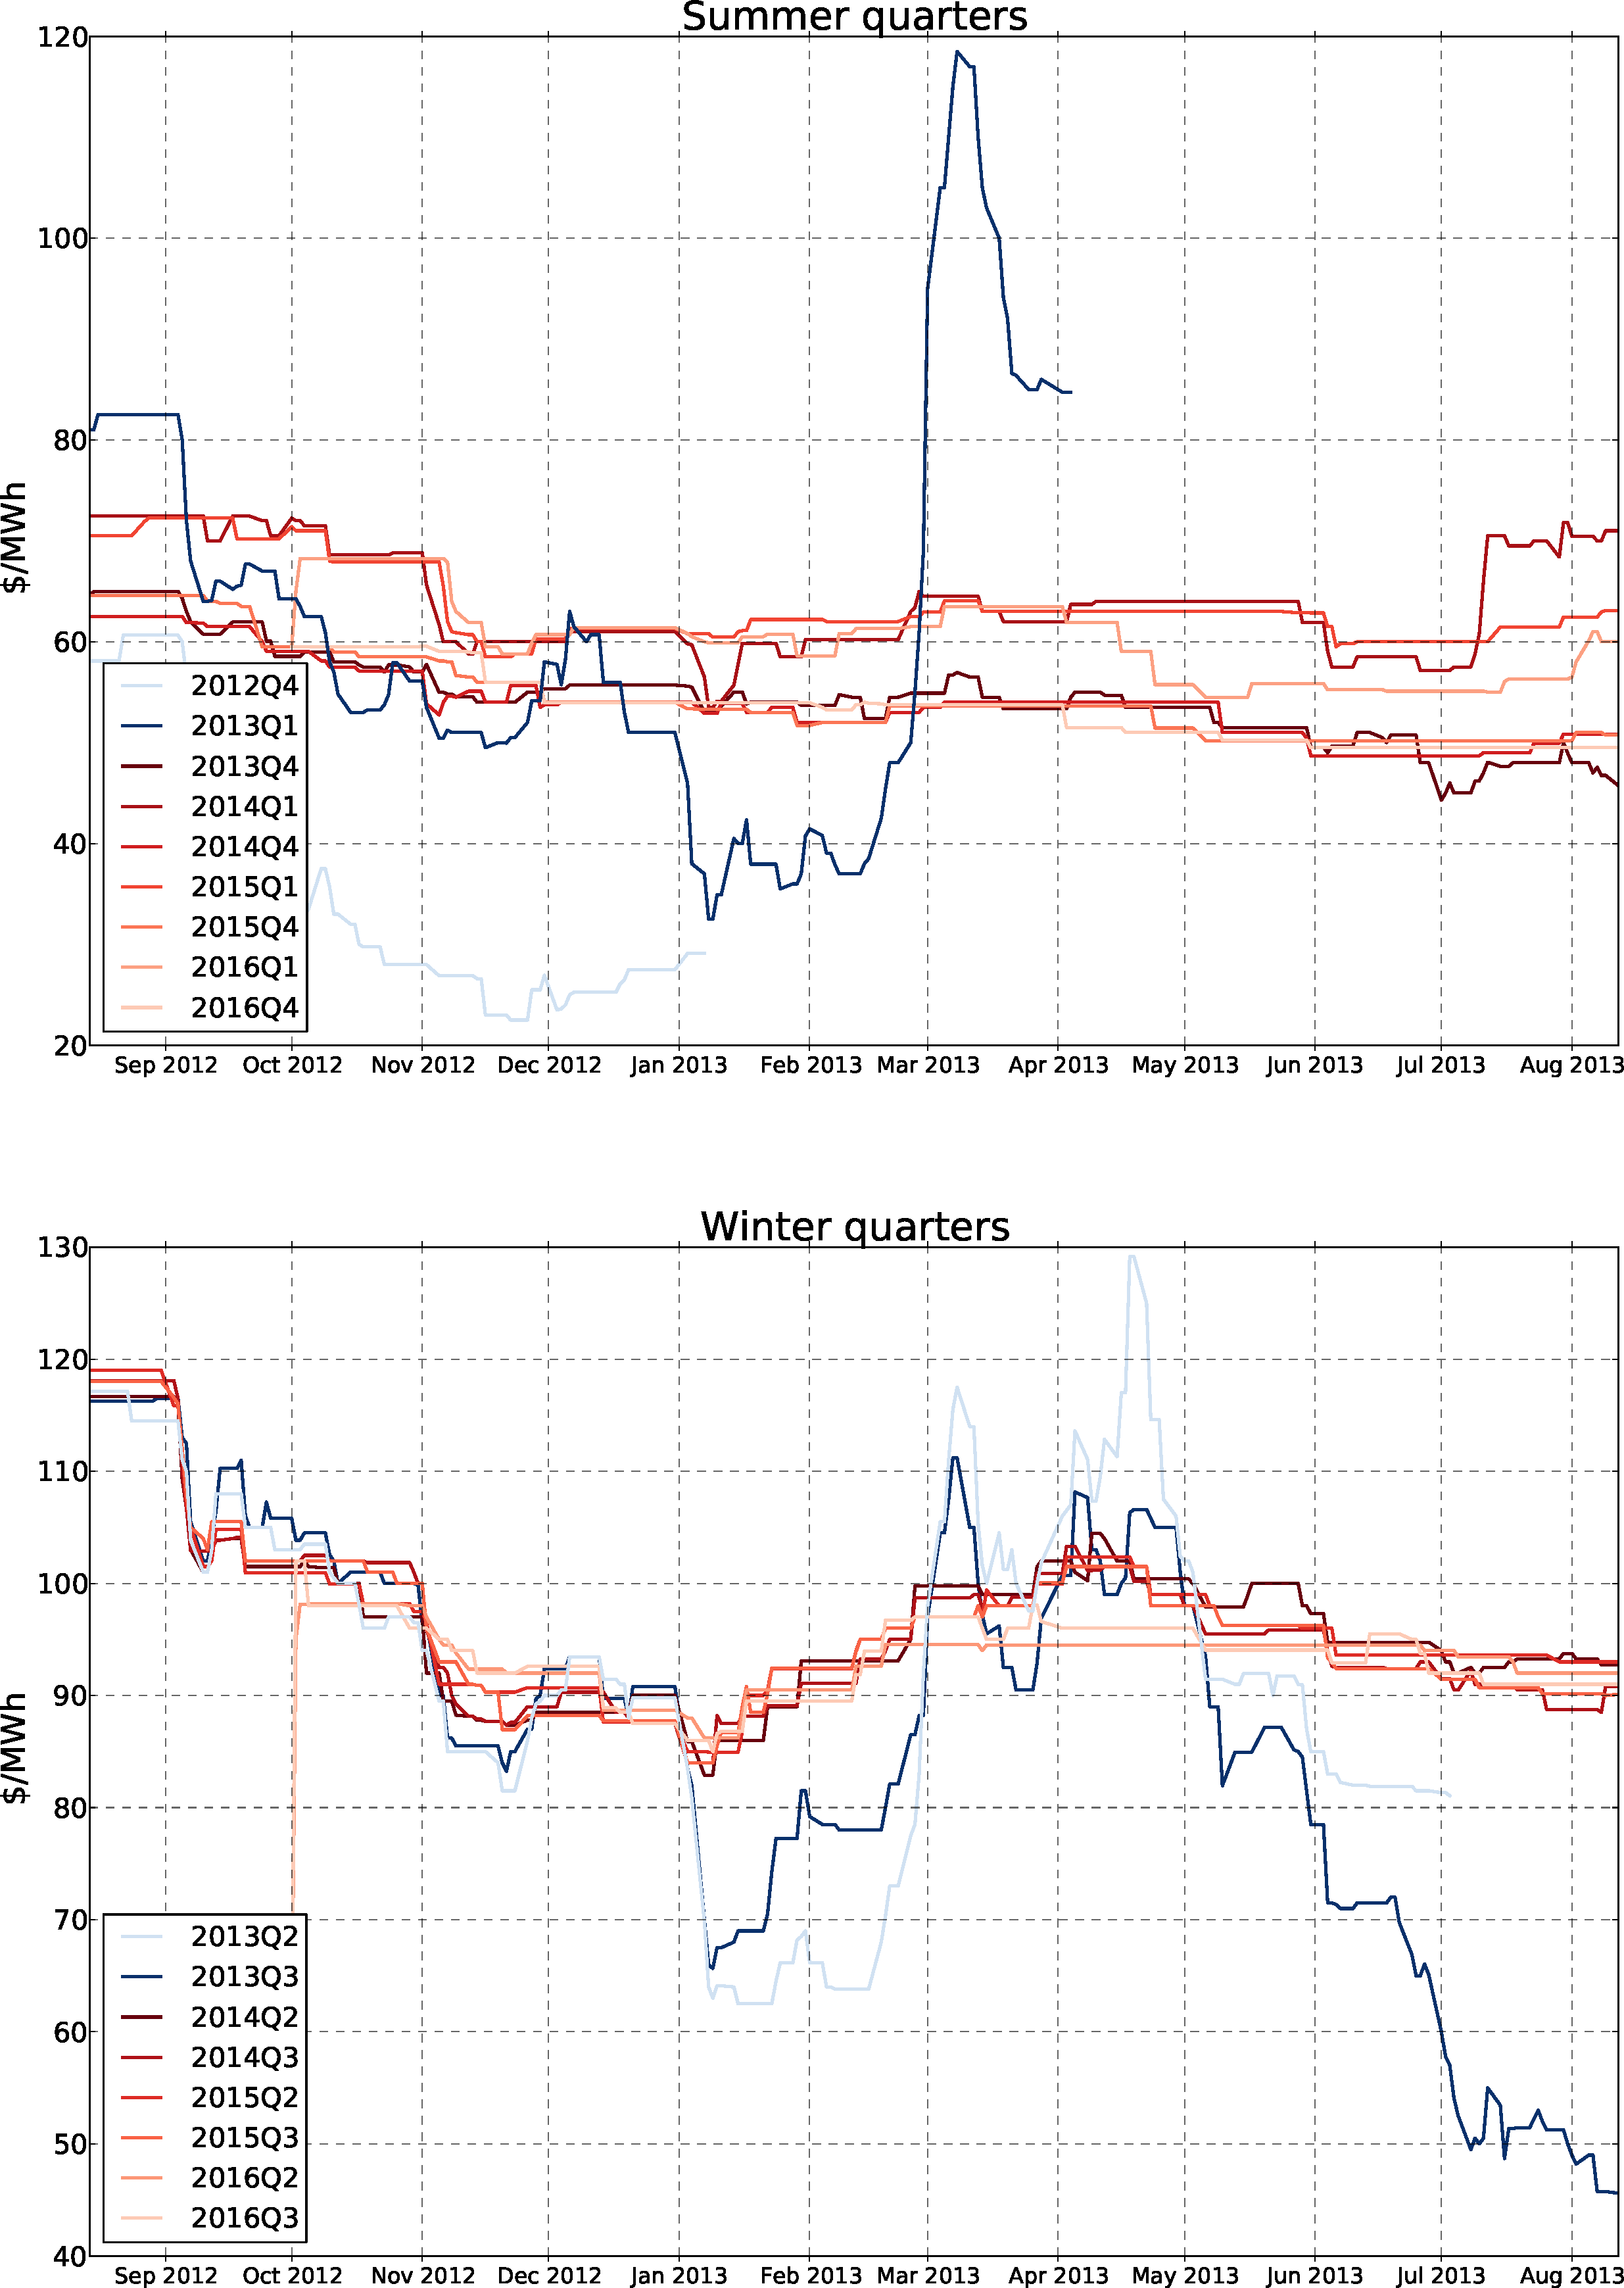
\includegraphics[max size={\textwidth}{0.9\textheight}]{/home/dave/python/reporting/figures/asx_ben_year.pdf}
\end{center}
\scriptsize Source: ASX \url{http://www.asx.com.au}

\subsection{Trends over last year - Benmore minus Otahuhu}

\begin{center}
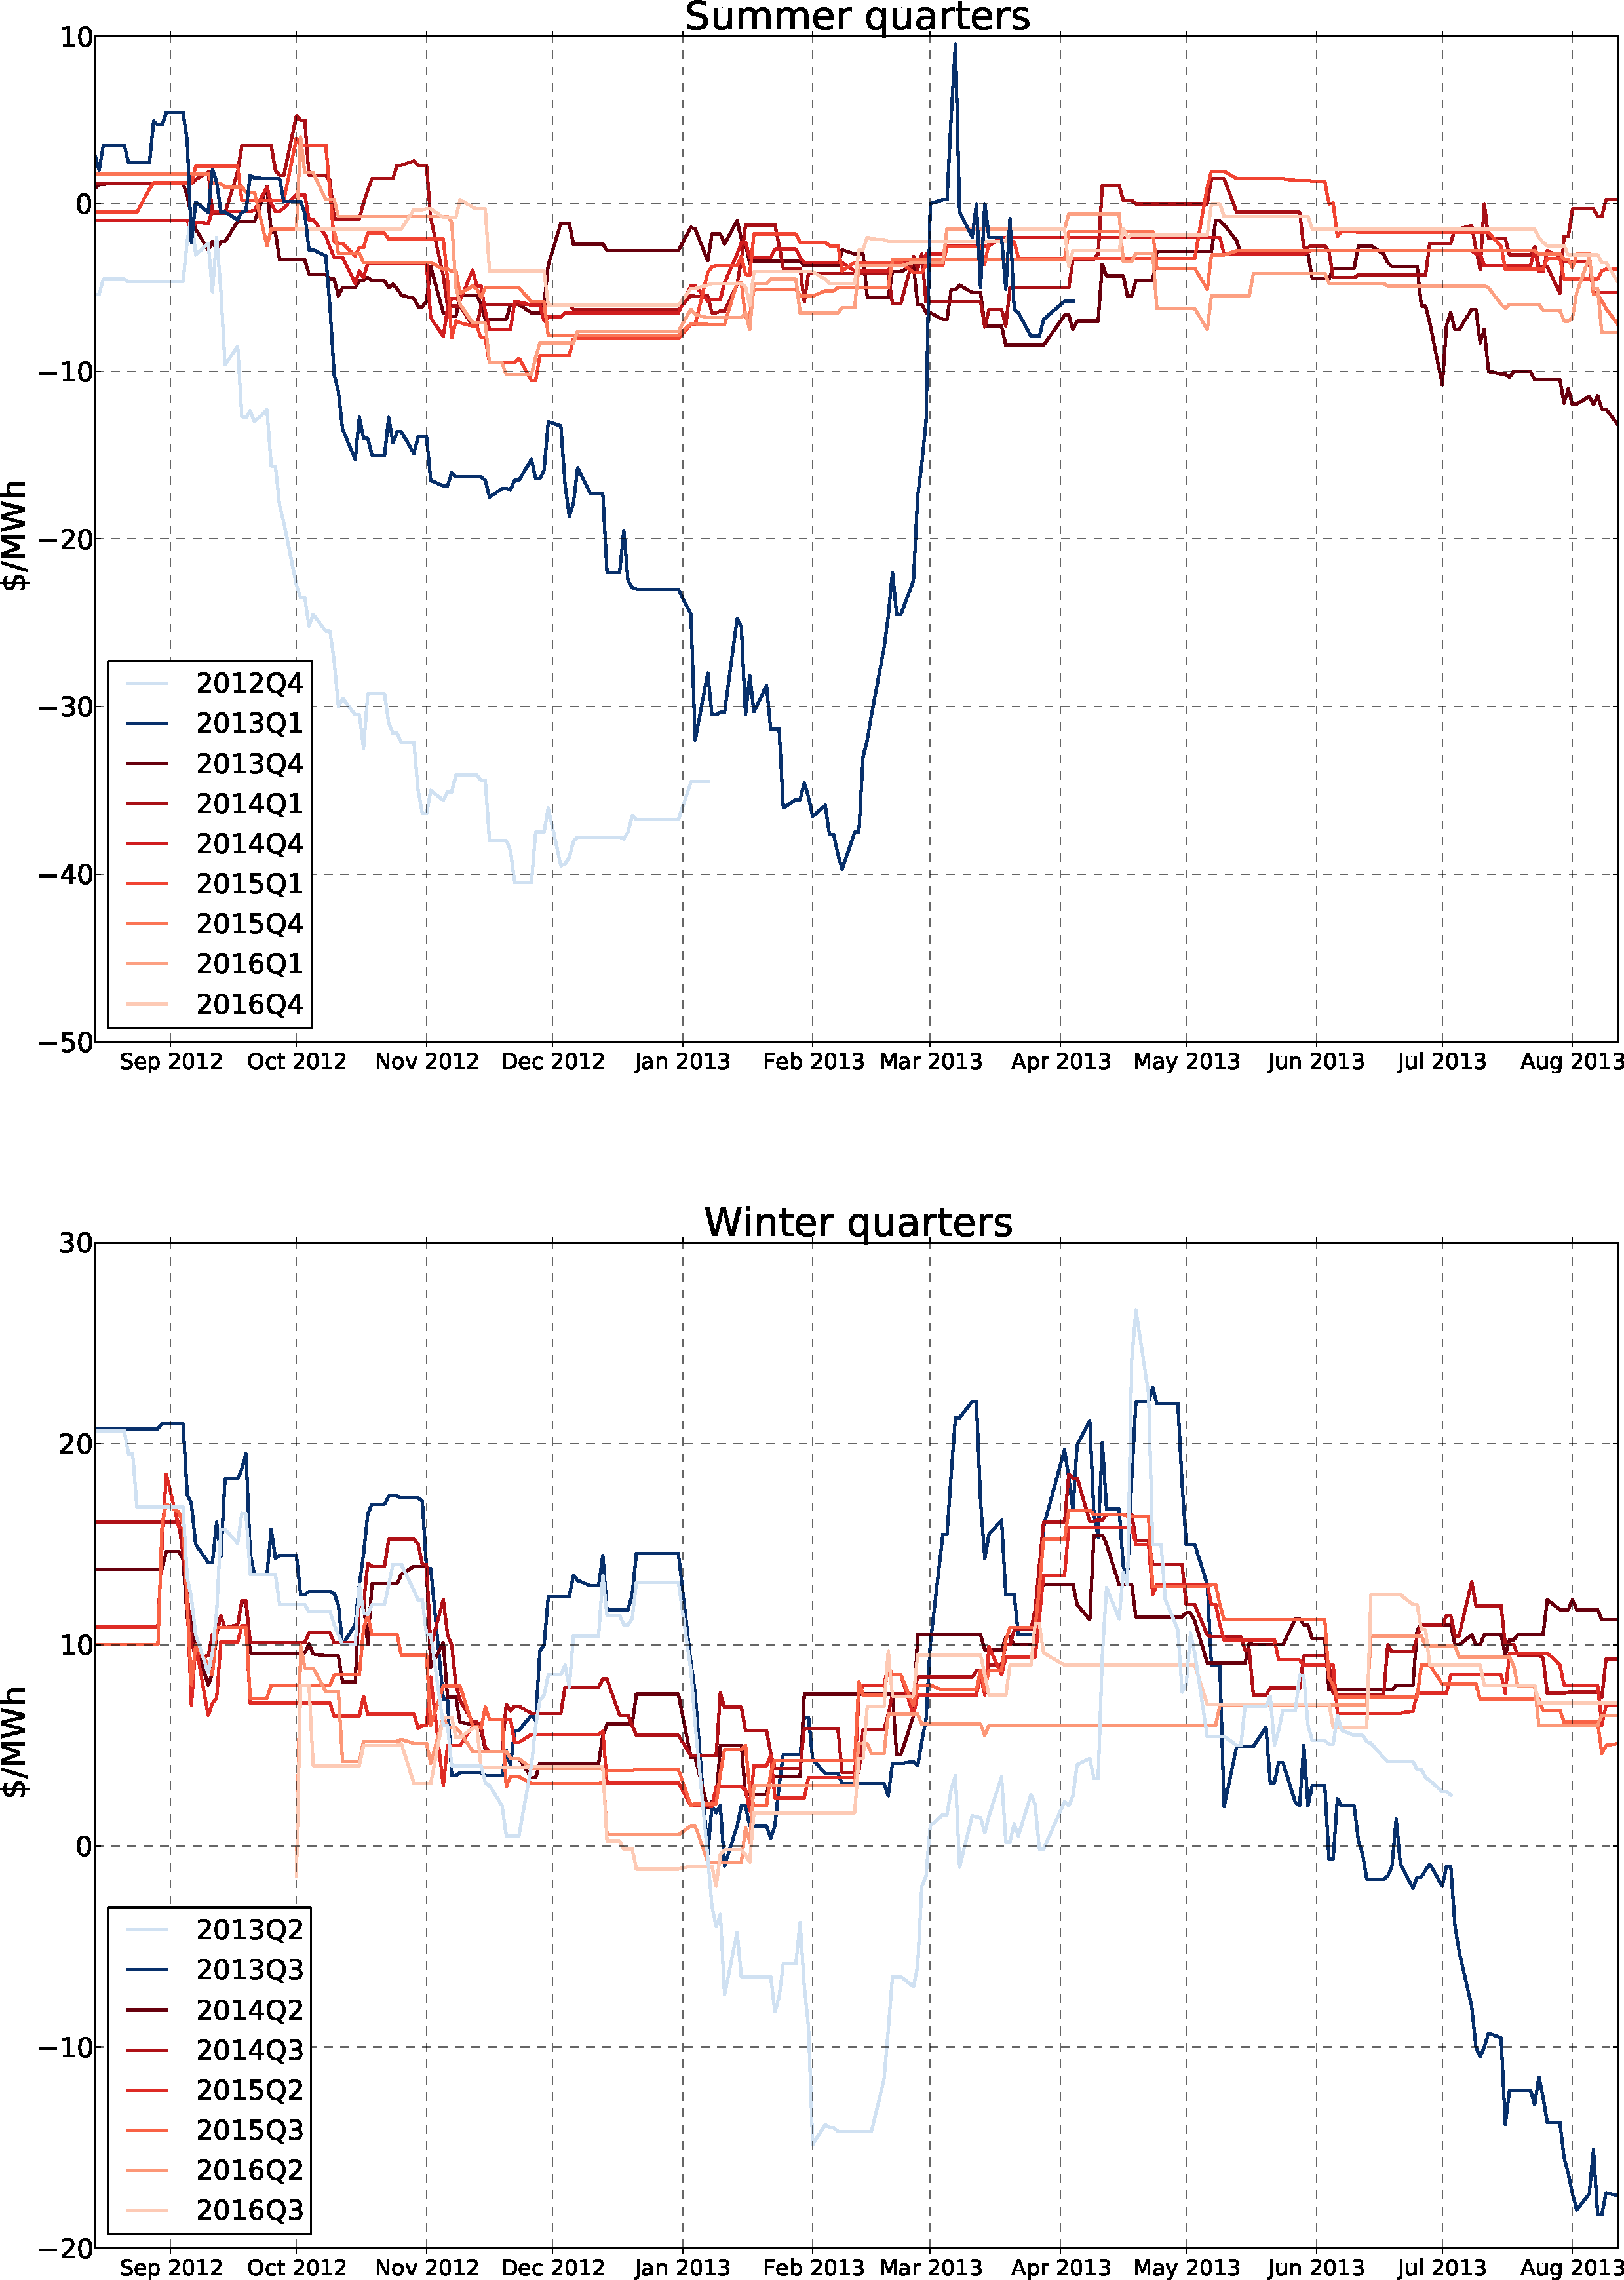
\includegraphics[max size={\textwidth}{0.9\textheight}]{/home/dave/python/reporting/figures/asx_ben_minus_ota_year.pdf}
\end{center}
\scriptsize Source: ASX \url{http://www.asx.com.au}

\end{document}

